\documentclass[10pt, conference]{IEEEtran}

\usepackage{cite}
\usepackage{url}
\usepackage{amsmath,amssymb,amsfonts}
\usepackage{algpseudocode}
\usepackage{algorithm}
\usepackage{graphicx}
\usepackage{textcomp}
\usepackage{xcolor}
\usepackage{booktabs}
\usepackage{makecell}
\usepackage[font=footnotesize,labelfont=bf]{subcaption}




\def\BibTeX{{\rm B\kern-.05em{\sc i\kern-.025em b}\kern-.08em
    T\kern-.1667em\lower.7ex\hbox{E}\kern-.125emX}}
\begin{document}

\title{Evaluating the Sensitivity of Isolation Forest Parameters in Anomaly Detection\\

}

\author{\IEEEauthorblockN{DT Nicolay 26296918}
\IEEEauthorblockA{\textit{Computer Science Division} \\
\textit{Stellenbosch University}\\
Stellenbosch, South Africa \\
26296918@sun.ac.za}
}

\maketitle

\begin{abstract}
TODO
\end{abstract}

\begin{IEEEkeywords}
TODO
\end{IEEEkeywords}

\section{Introduction}
% Start with purpose
Employing Isolation Forests to solve anomaly detection problems involves selecting numerous control parameters which affect the model's ability to correctly identify anomalies. When used properly, Isolation Forests are powerful tools with significant discriminative power, especially considering their simplicity.

% then what was done

% define "anomalies"

% main finding

% report structure description

\section{Background}
The theoretical background of Isolation Forests is presented in this section. The control parameters of the algorithm are also described.
\subsection{Isolation Forests}
% background inituition
% main idea
% algorithm?
The majority of existing model-based approaches to anomaly detection construct a profile of normal instances, then they identify instances that do not conform to this normal profile as anomalies \cite{iforest}. Liu et al. (2008) proposed a fundamentally different model-based method that explicitly isolates anomalies instead of profiles normal points, Isolation Forests. Here, isolation refers to separating an instance from the rest of the instances. This is ideal for an anomaly detection problem context, since anomalies are by nature sparse and diverse.

% iforest is bettern than statisitcal method, classification-based methods, clustering-based method (they all use normal )
Normal profile methods, since not optimised for anomaly detection, often lead to too many false positives or little to no anomalies detected at all. These methods are also constrained to low dimensional data and small data size since they require significant computational power. Isolation Forests, on the other hand, take advantage of anomaly datasets consisting of fewer observations for the target class, and anomalies having feature values distinct from the rest of the data. Due to the nature of anomaly observations, they are isolated closer to the root of the tree. This forms the foundation of isolation trees.

Isolation Forests involve an ensemble of isolation trees where the predicted anomalies are the observations with the shortest average paths across the trees. Using this model for anomaly detection involves two stages. The first stage constructs isolation trees by recursively partitioning. This training stage is described in Algorithm~\ref{alg:iforest} and Algorithm~\ref{alg:itree} \cite{iforest2}.

\begin{algorithm}[H]
	\caption{iForest($X$, $t$, $\psi$)}
	\label{alg:iforest}
	\begin{algorithmic}[1]
		\Require $X$ -- input data, \ $t$ -- number of trees, \ $\psi$ -- subsampling size
		\Ensure A set of $t$ isolation trees
		\State Initialize $\text{Forest} \gets \emptyset$
		\For{$i = 1$ to $t$}
		\State $X' \gets \text{sample}(X, \psi)$
		\State $\text{Forest} \gets \text{Forest} \cup \text{iTree}(X')$
		\EndFor \\
		\Return $\text{Forest}$
	\end{algorithmic}
\end{algorithm}

The iTree algorithm recursively partitions the dataset by randomly selecting a feature and a random split value until the data can no longer be divided. The resulting tree structure isolates individual points, where anomalies tend to have shorter average path lengths because they are easier to isolate.

\begin{algorithm}[H]
	\caption{iTree($X'$)}
	\label{alg:itree}
	\begin{algorithmic}[1]
		\Require $X'$ -- input data  
		\Ensure an isolation tree
		\If{$X'$ cannot be divided}
		\Return $\text{exNode}\{\text{Size} \leftarrow |X'|\}$
		\Else
		\State Let $Q$ be the list of attributes in $X'$
		\State Randomly select an attribute $q \in Q$
		\State Randomly select a split point $p$ between the max and min values of attribute $q$ in $X'$
		\State $X_l \gets \text{filter}(X', q < p)$
		\State $X_r \gets \text{filter}(X', q \ge p)$
		\Return $\text{inNode}\{$ \\
		\hspace*{1.5em} $\text{Left} \leftarrow \text{iTree}(X_l),$ \\
		\hspace*{1.5em} $\text{Right} \leftarrow \text{iTree}(X_r),$ \\
		\hspace*{1.5em} $\text{SplitAtt} \leftarrow q,$ \\
		\hspace*{1.5em} $\text{SplitValue} \leftarrow p\}$ 
		\EndIf
	\end{algorithmic}
\end{algorithm}


% TODO add some more commmentary from looking at sklearn docs


\subsection{Control Parameters}
% original paper parms num est & max samples
There are five control parameters to consider namely: the number of estimators, the maximum samples, the contamination, the maximum features, and whether to first bootstrap sample.

The number of estimators parameter determines the number of base trees in the ensemble. This parameter is denoted by $t$ in Algorithm~\ref{alg:iforest}. The performance of Isolation Forests converges quickly with a very small number of trees \cite{iforest}.


The maximum samples parameter describes the number of sample observations to draw from the training data for each base estimator. This subsampling size is denoted by $\psi$ in Algorithm~\ref{alg:iforest}. Only a small sampling size is required to achieve high detection performance with high efficiency \cite{iforest}. Setting $\psi$ to 256 often suffices for anomaly detection across a wide range of data \cite{iforest2}.

% contamination additional parameter
Contamination refers to the proportion of anomalies present in the dataset. It is defined as the number of anomalies divided by total number of observations. When set to a specific value between 0 and 0.5, it determines the threshold on the anomaly scores such that approximately that fraction of the training samples are labelled as outliers. In the original paper, the threshold is automatically fixed at an offset of -0.5, following the original Isolation Forest formulation, where inliers typically yield scores near 0 and outliers near -1, allowing the model to separate them without prior knowledge of the true contamination level. Since this parameter directly influences the threshold for anomaly detection, mis-tuning will directly increase false positives or false negative rates.

% max features additional parameter
The maximum features describes how many features are selected at random before tree construction, and are used to train each base estimator. Introducing randomness can help with with high-dimensional data, but may increase instability if set too low.

% bootstrap additional parameter 
The bootstrap parameter controls the manner in which sample observations are drawn for each tree. This determines whether sampling is done with or without replacement. That is, sub-sample $X'$ is randomly sampled with or without replacement in Algorithm~\ref{alg:iforest} from $X$. Bootstrap resampling can lead to marginal improvements across classification metrics \cite{Choi2025Impact}.

\subsection{Evaluation Stage}
For this stage, a single path length $h(\boldsymbol{x})$ is computed by counting the number of edges from the root node to an external node as an instance $\boldsymbol{x}$ traverse each iTree. There is a predefined height limit, \textit{hlim}, that when reached, the algorithm returns the value $e$ plus an adjustment $c(Size)$. This process is described in Algorithm~\ref{alg:pathlength} \cite{iforest2}. The worst case time complexity of the evaluation stage for a dataset size $n$ is $O(nt \psi)$.

\begin{algorithm}[H]
	\caption{PathLength($\boldsymbol{x}, T, h_{lim}, e$)}
	\label{alg:pathlength}
	\begin{algorithmic}[1]
		\Require $\boldsymbol{x}$ -- an instance; $T$ -- an iTree; $h_{lim}$ -- height limit; $e$ -- current path length (initialized to 0 when first called)
		\Ensure Path length of $\boldsymbol{x}$
		\If{$T$ is an external node \textbf{or} $e \ge h_{lim}$}
		\State \Return $e + c(T.\text{size})$ \Comment{$c(\cdot)$ is defined in Equation (1)}
		\Else
		\State $a \gets T.\text{splitAtt}$
		\If{$x_a < T.\text{splitValue}$}
		\State \Return $\text{PathLength}(\boldsymbol{x}, T.\text{left}, h_{lim}, e + 1)$
		\Else
		\State \Return $\text{PathLength}(\boldsymbol{x}, T.\text{right}, h_{lim}, e + 1)$
		\EndIf
		\EndIf
	\end{algorithmic}
\end{algorithm}

The anomaly score $s(\boldsymbol{x}, \psi)$ for instance $\boldsymbol{x}$ is computed using

\begin{equation}
	s(\boldsymbol{x} \psi) = 2^{- \frac{E(h(\boldsymbol{x}))}{c(\psi)}},
\end{equation}

where $c(\psi)$ is the average path length of unsuccessful searches and $E(h(\boldsymbol{x}))$ is the average depth from the forest of isolation trees. If the score of an observation $s$ is close to 1, the observation is an anomaly. If an observation has a score much smaller than 0.5, then it is regarded as a normal instance. However, if all observations return a score of approximately 0.5, then there are no distinct anomalies.

Two effects occur when the model cannot correctly identify anomalous instances properly. Swamping occurs when wrongly identifying normal instances are classified as anomalies, typically occurring when normal instances are too close to anomalies. This increases the number of partitions required to isolate anomalies, making them less distinguishable. Masking occurs when the forest fails to identify anomalies because too many anomalies exist in a cluster. This makes them conceal one another. In this case, the path lengths required to isolate each anomaly also increases.


\section{Implementation}
The approach, tools, and experimental set-up of the Isolation Forest control parameter tests are all described in this section.
\subsection{Tools and Libraries}
This implementation was created using Python. NumPy\cite{harris2020array} is used for numerical computations. Pandas\cite{reback2020pandas} is used for data manipulation and analysis. Matplotlib\cite{Hunter:2007} is used for data visualisation and plotting. Scikit-learn\cite{scikit-learn} was used extensively fo modelling, evaluation, and the evaluation metrics.
\subsection{Isolation Forest Algorithm}
% brief recap alg
The Scikit-learn library \cite{scikit-learn} implementation of the Isolation Forest algorithm described in the background section is used to detect anomalies across three varied datasets. This implementation returns the anomaly score for each observation. The path length to an observation in the a tree, averaged over a forest of isolation trees, is used as a measure of normality and the decision function. When the Isolation Forest collectively produces shorter path length for a particular observation, it is likely to be an anomaly. The maximum depth of each tree is $\lceil log_2(n) \rceil$ where $n$ is the number of samples used to build the tree.

% our setup
A custom framework is built around the base Isolation Forest implementation to track evaluation metric means and their standard deviations over a specified number of runs. The control parameter comparisons are split into two sections. First, the analysis is conducted on each dataset individually and all results are saved. Plots and statistical tests are performed for the individual datasets to compare the control parameters. Second, the results from the individual datasets tests are compared across datasets separately to analyse the data-dependent effects.



\subsection{Experimental Setup}
A random seed of 12 is used for all stochastic procedures to ensure reproducibility. All tests are conducted on a Fedora Linux 41 system with a 13th Gen Intel Core i3-13100 CPU with 16 GiB of memory. The computationally significant portions of the algorithm are running the algorithm with a large ensemble size and also a large parameter grid for some parameter combinations. The code for this paper is available on GitHub \cite{github}.
\section{Empirical Process}
% 20 MARKS
The datasets and their rationale are described in this section. This is followed by an explanation of the evaluation metrics used along with the experimental design.
\subsection{Datasets}

% table summary
% rationale for selection
The datasets used for control parameter evaluation are described in Table~\ref{tab:datasets} and are all sourced from ADBench \cite{han2022adbench}. These datasets provide a variety in the number of observations, features, anomaly rate, and the difficulty of the anomaly detection problem. This enabled a thorough and balanced representation of the performance of the control parameters in different problem settings.
\begin{table}[H]
	\centering
	\caption{Summary of Datasets Used}
	\begin{tabular}{|l|r|r|r|l|}
		\hline
		\textbf{Dataset} & \textbf{Observations} & \textbf{Features} & \textbf{\shortstack{Anomaly\\Rate (\%)}} & \textbf{Domain} \\ \hline
		Shuttle  & 49,097  & 9  & 7.15  & Astronautics \\ \hline
		Campaign & 41,188  & 62 & 11.27 & Finance \\ \hline
		Fraud    & 284,807 & 29 & 0.17  & Finance \\ \hline
	\end{tabular}
	\label{tab:datasets}
\end{table}



\subsection{Evaluation Metrics}
% metrics and justification
Given the nature of anomaly detection as an imbalanced classification problem, metrics must account for the typically small proportion of anomalies in real-world datasets, as evidenced by the 0.17\% anomaly rate in the \textit{fraud} dataset compared to 11.27\% in \textit{campaign}. The F1-score served as the primary performance indicator, providing a balanced measure between precision and recall. Precision quantified the proportion of correctly identified anomalies among all flagged instances, which is critical in applications where false alarms incur significant investigation costs. Recall measured the proportion of true anomalies successfully detected, representing the algorithm's sensitivity to anomalous patterns. Both metrics are essential as they capture the trade-off inherent in anomaly detection: aggressive detection (high recall) risks overwhelming analysts with false positives, while conservative detection (high precision) may miss critical anomalies.

ROC-AUC (Receiver Operating Characteristic Area Under Curve) and PR-AUC (Precision-Recall Area Under Curve) evaluated the model's ability to rank anomalies correctly across different decision thresholds. ROC-AUC assesses overall discriminative power, while PR-AUC is particularly informative for imbalanced datasets as it focuses on performance in the positive (anomaly) class. These metrics were computed using the anomaly scores from Isolation Forest's \texttt{score\_samples()} method, which provides a continuous ranking rather than binary classifications.

Since Isolation Forests are stochastic in nature with regards to feature selection during tree construction, performance does vary between runs.The Jaccard similarity coefficient was used to measure the performance consistency between runs. Training time and memory usage were also tracked to assess the scalability and computational resource management. The average path length statistic was also monitored.
\subsection{Experimental Design}
\subsubsection{Single-Parameter Analysis}
%Methodology: Vary one parameter while holding others at defaults
Each control parameter was individually varied whilst holding all the others at their base parameters. These base parameters are 100 estimators, 256 maximum samples, the actual contamination percentage of the dataset, all features included and bootstrap sampling disabled. For each configuration, 10 runs were performed with the random seed incremented for each run. The mean, minimum, maximum and standard deviation of all the performance metrics were recorded.

% n est
For the number of estimators in the ensemble, the range considered was $n_\text{estimators} \in \{1,2,...,25,50,75,100,125,175,200\}$. Originally, a much broader range with larger intervals up to 2000 was considered. However, convergence analysis revealed that the ensemble often converged before 100/200 estimators, therefore, a narrower set of values was considered to more closely monitor trends. The range for the maximum samples parameter was $n_\text{max samples} \in \{4,8,12,16,20,24,28,32,64,128,256, 512\}$. The smaller interval points captured more specific information about where the model converged, and the larger gaps considered the larger parameter values to obtain a broader view of the performance. The contamination parameter was considered over the values $\text{contamination} \in \{0.01, 0.02, 0.03, 0.05, 0.07, 0.10, 0.15, 0.20, 0.25, 0.30\}$. The contamination parameter is obviously problem dependent, and, in a true unsupervised learning scenario, unknown. The maximum features parameter was varied linearly from 1 up to the total number of available features (capped at 20) using integer increments. Bootstrap sub-sampling was also considered.

Three or four plots were created for each parameter experiment. Most notably, the convergence plot including F1-score, precision, and recall against the parameter value was created. This plot included the standard deviation in addition to the mean to illustrate the variability over the 10 runs. The training time scaling was plotted by considering the training time against the parameter plotted on a log-log scale. For parameters affecting the precision-recall balance (such as contamination and maximum samples), precision-recall curves were constructed to visualize the trade-offs inherent in different parameter configurations.

The coefficient of variation was computed for the F1-score across the 10 runs to quantify stability, with lower CV values indicating more consistent performance. For the contamination parameter specifically, calibration curves were generated to assess whether the specified contamination level reliably controlled the proportion of instances flagged as anomalies, providing insight into the parameter's predictive calibration.

\subsubsection{Multi-Parameter Interaction Analysis}
Interactions between the maximum features and number of estimator parameters were considered by running all the combinations of the previously described maximum feature range and the number of estimators in intervals of three from one to 25. For example, for the \textit{shuttle} dataset, $9 \times 9 = 81$ combinations were considered. The training time and F1-scores were plotted in a heat map to investigate any correlations. The interaction between the contamination parameter and bootstrap parameter was also investigated.
\subsubsection{Cross-Dataset Comparison}
The convergence curves along with the training times further were analysed across the various datasets in the same plots. This enabled the identification of data specific trends. The variation across runs was also plotted across the various datasets in order to compare the stability of the application to the different datasets.





\section{Results \& Discussion}
% intro
The observed effects of the control parameters are described in this section. An analysis of the plots and experiment results is presented, followed by practical guidelines for the selection of the parameters for various applications.
\subsection{Number of Estimators}
\subsubsection{Performance Convergence}
% show multi plot
Generally, the performance reported by the F1-score indicated that the model converged with 50 estimators in the ensemble. This is illustrated in Figure~\ref{fig:n_estimators_f1}. The  datasets reported quite different F1-scores after convergence, which showed the varying complexity of the anomaly detection problems in each of the datasets. This is observed in Figure~\ref{fig:n_estimators_campaign} and Figure~\ref{fig:n_estimators_fraud}. For the fraud dataset, the F1-score only fully plateaued after 125 estimators were used in the ensemble. 

It can therefore be concluded that if 125 estimators are used, the model will likely converge. For computationally constrained circumstances, as few as 25 estimators will suffice for most use cases.
\begin{figure}[H]
	\centering
	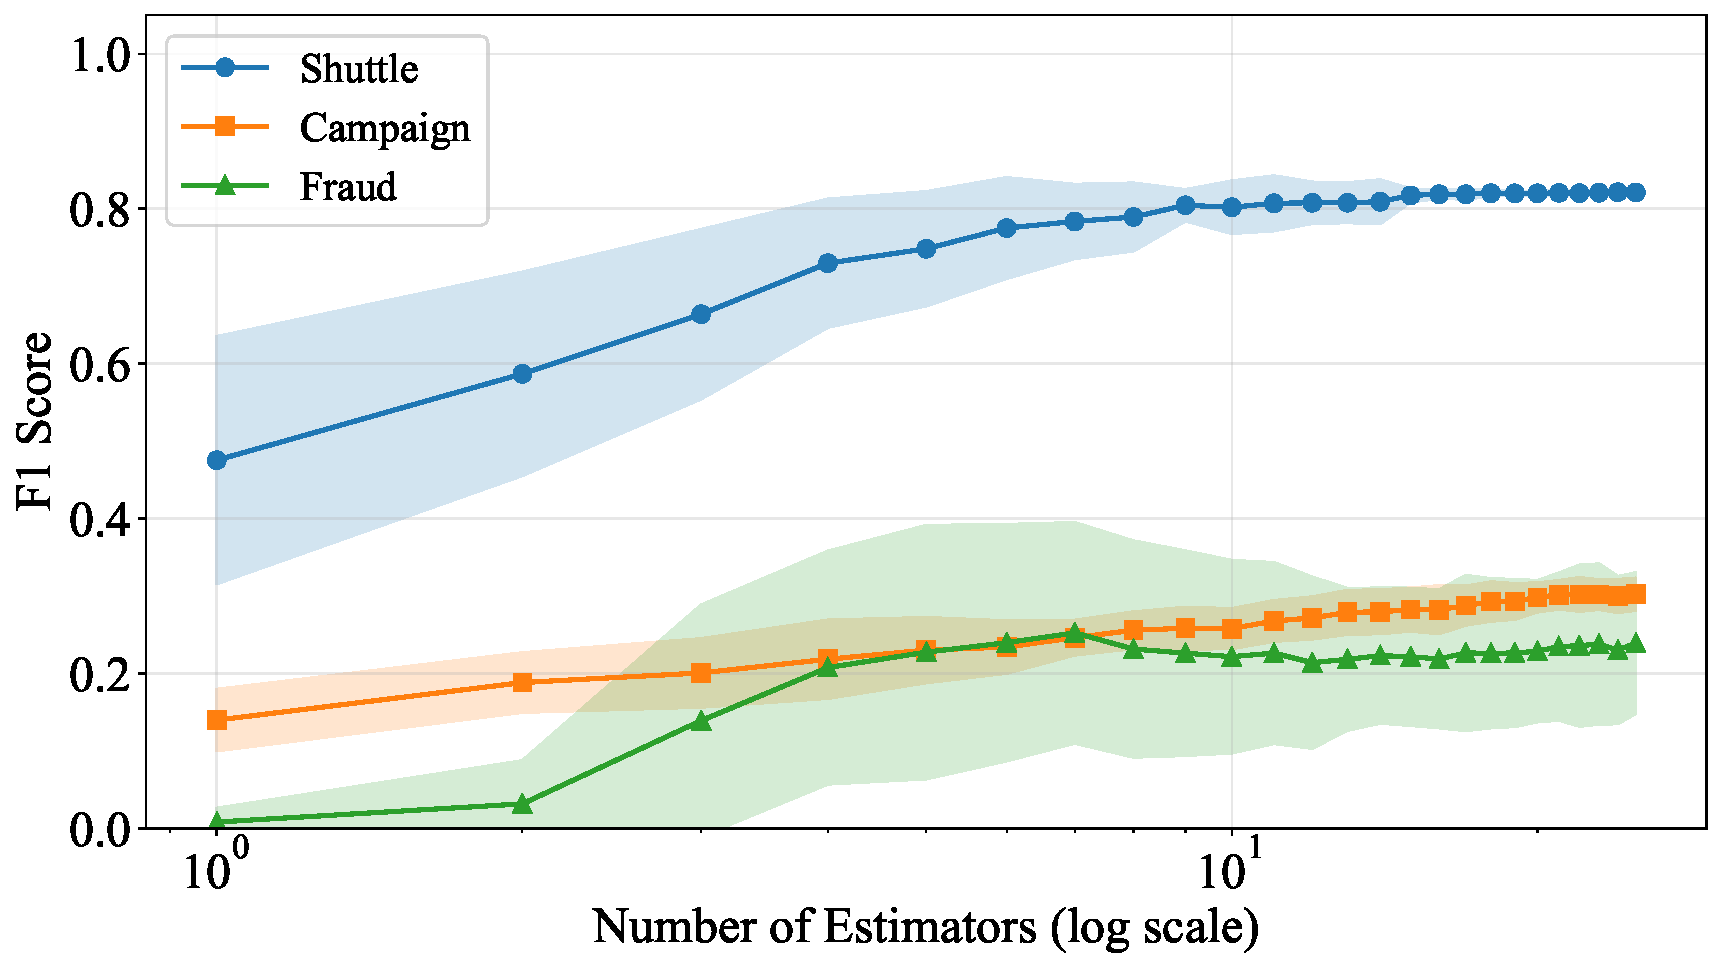
\includegraphics[width=0.95\linewidth]{../results/multi_dataset/n_estimators_f1.pdf}
	\caption{F1-score performance across datasets for varying numbers of estimators.}
	\label{fig:n_estimators_f1}
\end{figure}


% refer to appendix

% observations - where do we plataeu

% dataset complexity and reqiured ensemble size

\subsubsection{Stability and Variance Reduction}
% coef variation vs n est
% observe exponetial decay in variance?
The coefficient of variation calculated by dividing the mean F1-score by the F1-score standard deviation only fully stabilised at 125 estimators for the campaign and fraud datasets, but before 25 for the shuttle dataset. This stability is shown in in Figure~\ref{fig:n_estimators_var} for the campaign dataset and Figure~\ref{fig:n_estimators_var_shuttle} and Figure~\ref{fig:n_estimators_var_fraud} for the other two. 

This behaviour aligns with the Law of Large Numbers: as the number of estimators increases, the random variation in individual model predictions averages out, causing the ensemble’s F1-score to converge towards its expected value. Consequently, the variance of the mean decreases approximately as 
$1/n$, leading to the observed stability beyond 125 estimators. A lower coefficient of variation means the model is more reliable and therefore a higher number of estimators should be used in a case where consistent performance is critical such as fraud detection systems or campaign targeting pipelines where unstable predictions could lead to significant financial or reputational loss.

\begin{figure}[H]
	\centering
	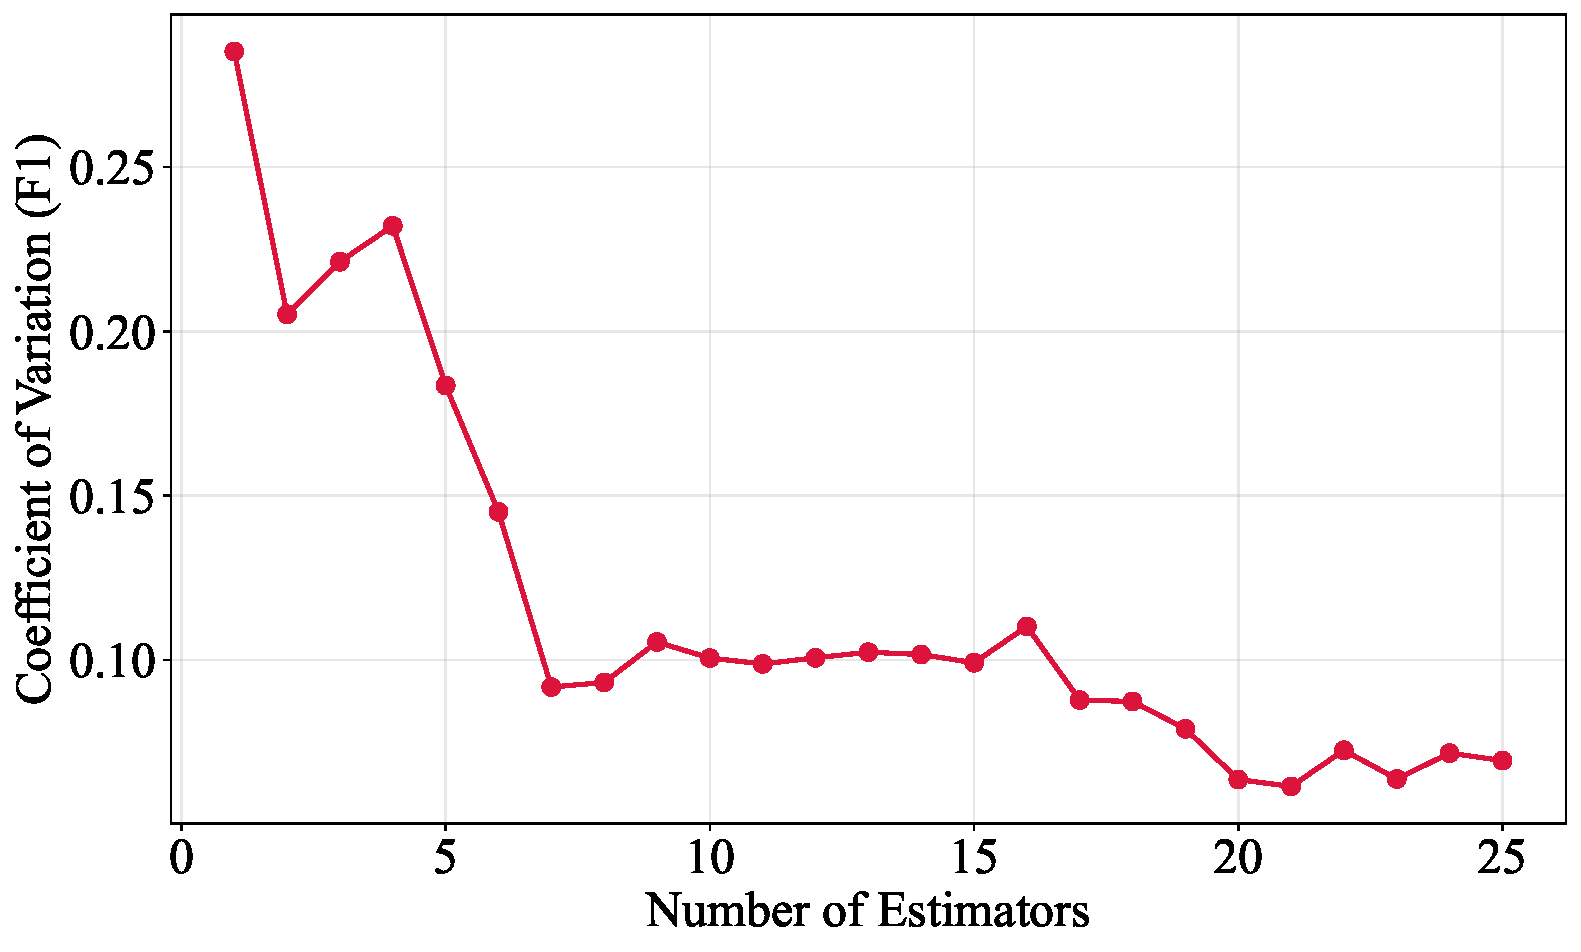
\includegraphics[width=0.95\linewidth]{../results/campaign/n_estimators/stability_analysis.pdf}
	\caption{Stability analysis of campaign dataset.}
	\label{fig:n_estimators_var}
\end{figure}

\subsubsection{Computational Efficiency}
% f1 vs training time scatter
The training time of the model scaled linearly as the number of estimators was increased. This relationship, observed in Figure~\ref{fig:n_estimators_tt}, indicates that the per-estimator training cost is approximately constant across the range of the number of estimators. Also, there was no significant overhead or parallelisation bottleneck as the ensemble grows. As expected, the fraud dataset maintained the highest training time throughout the experiment since it contains the most observations.
\begin{figure}[H]
	\centering
	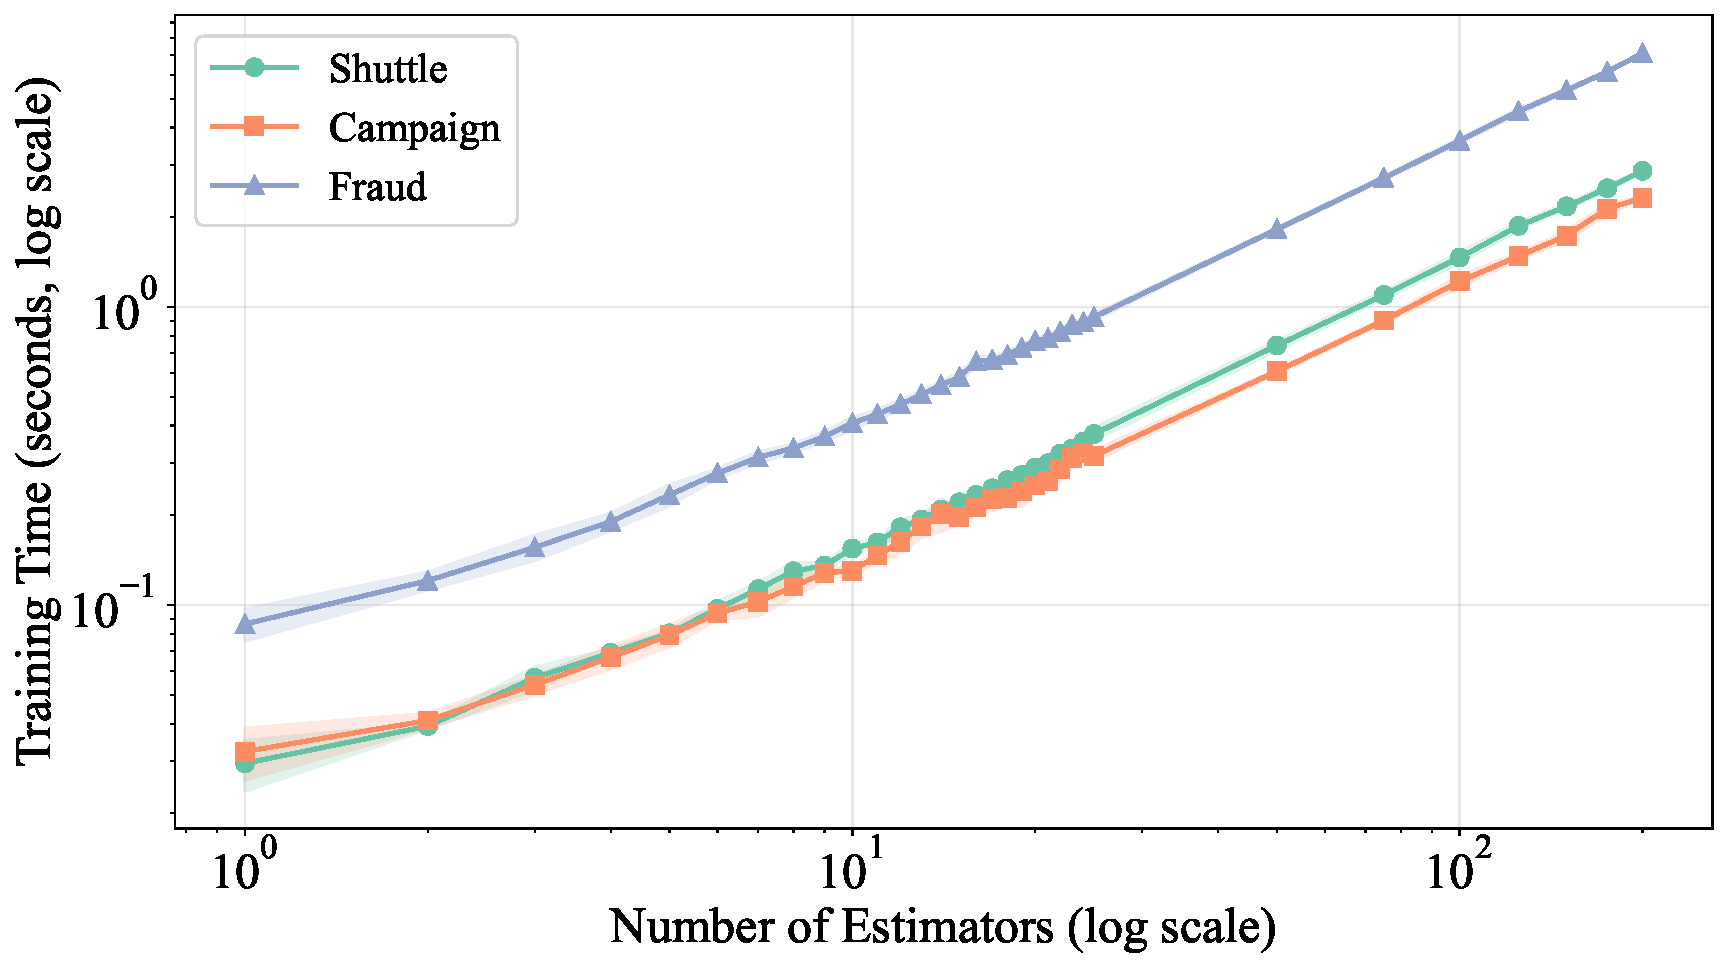
\includegraphics[width=0.95\linewidth]{../results/multi_dataset/n_estimators_training_time.pdf}
	\caption{Training time across increasing number of estimators.}
	\label{fig:n_estimators_tt}
\end{figure}

% sweet spot observe
%give practical recommendation
% when to use larger

\subsection{Maximum Samples}
\subsubsection{Performance vs. Subsample size}
% fig f1 all cs max samples
The parameter value of 256 commonly recommended \cite{iforest2} showed impressive performance for the shuttle dataset. That is , the F1-score peaked at about this number of samples seen in Figure~\ref{fig:max_samples_all}. However, for the more complex fraud dataset, the F1-score was still gradually increasing even as the maximum samples approached 512. This increase was due to \textit{both} precision and recall improving as illustrated in Figure~\ref{fig:max_samples_fraud}. Therefore, a value of 256 is often sufficient to gain the majority of the predictive power of the Isolation Forest model. However, it should be acknowledged that small increases in performance can still be found at larger values for more complex datasets. This trend reflects the classic bias–variance trade-off, where smaller subsample sizes introduce higher bias (underfitting) while larger ones reduce bias but increase variance, leading to diminishing returns beyond a certain point. The drop in F1-score beyond 256 samples for the shuttle dataset suggests swamping, where excessive subsampling caused normal points to be incorrectly isolated as anomalies, degrading overall performance.
\begin{figure}[H]
	\centering
	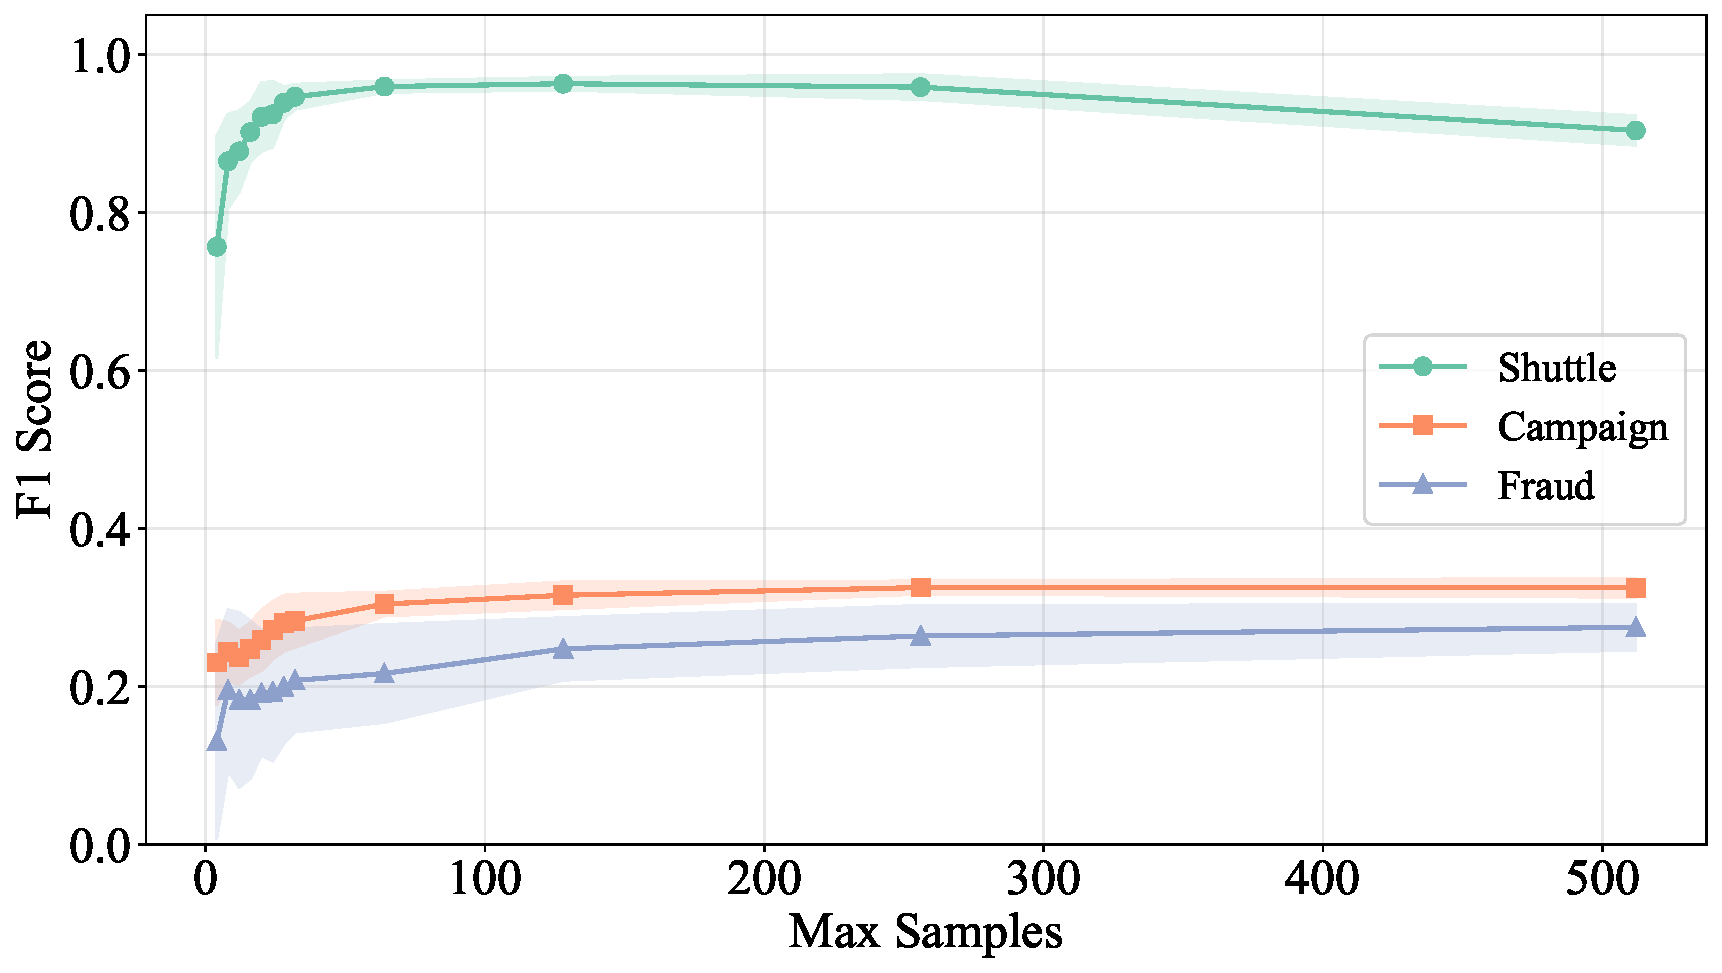
\includegraphics[width=0.95\linewidth]{../results/multi_dataset/max_samples_f1.pdf}
	\caption{Performance with increasing values of maximum samples parameter.}
	\label{fig:max_samples_all}
\end{figure}
% observe is auto optimal
% data specific patterns
% discuss bias variance tradoff
%Large samples → swamping (anomalies hidden in normal data)

\subsubsection{Swamping Effect Analysis}
% observe large samples boos recal but hurt precision, small sames opposive
% when does swamping become bad
% mechanism: small samples isolate anomalies faster
% fig precision recall curves
In the case of the shuttle dataset, the swamping effect occured after the parameter is set to 256, where the F1-score sharply drops from 0.9588 to 0.9039. This decline indicates that as the Isolation Forest begins to use too many samples, it starts isolating normal instances as anomalies, effectively “swamping” the true outliers within an overfitted model that loses its ability to clearly separate normal and anomalous points. This effect is also illustrated in Figure~\ref{fig:max_samples_shuttle}.

\begin{figure}[H]
	\centering
	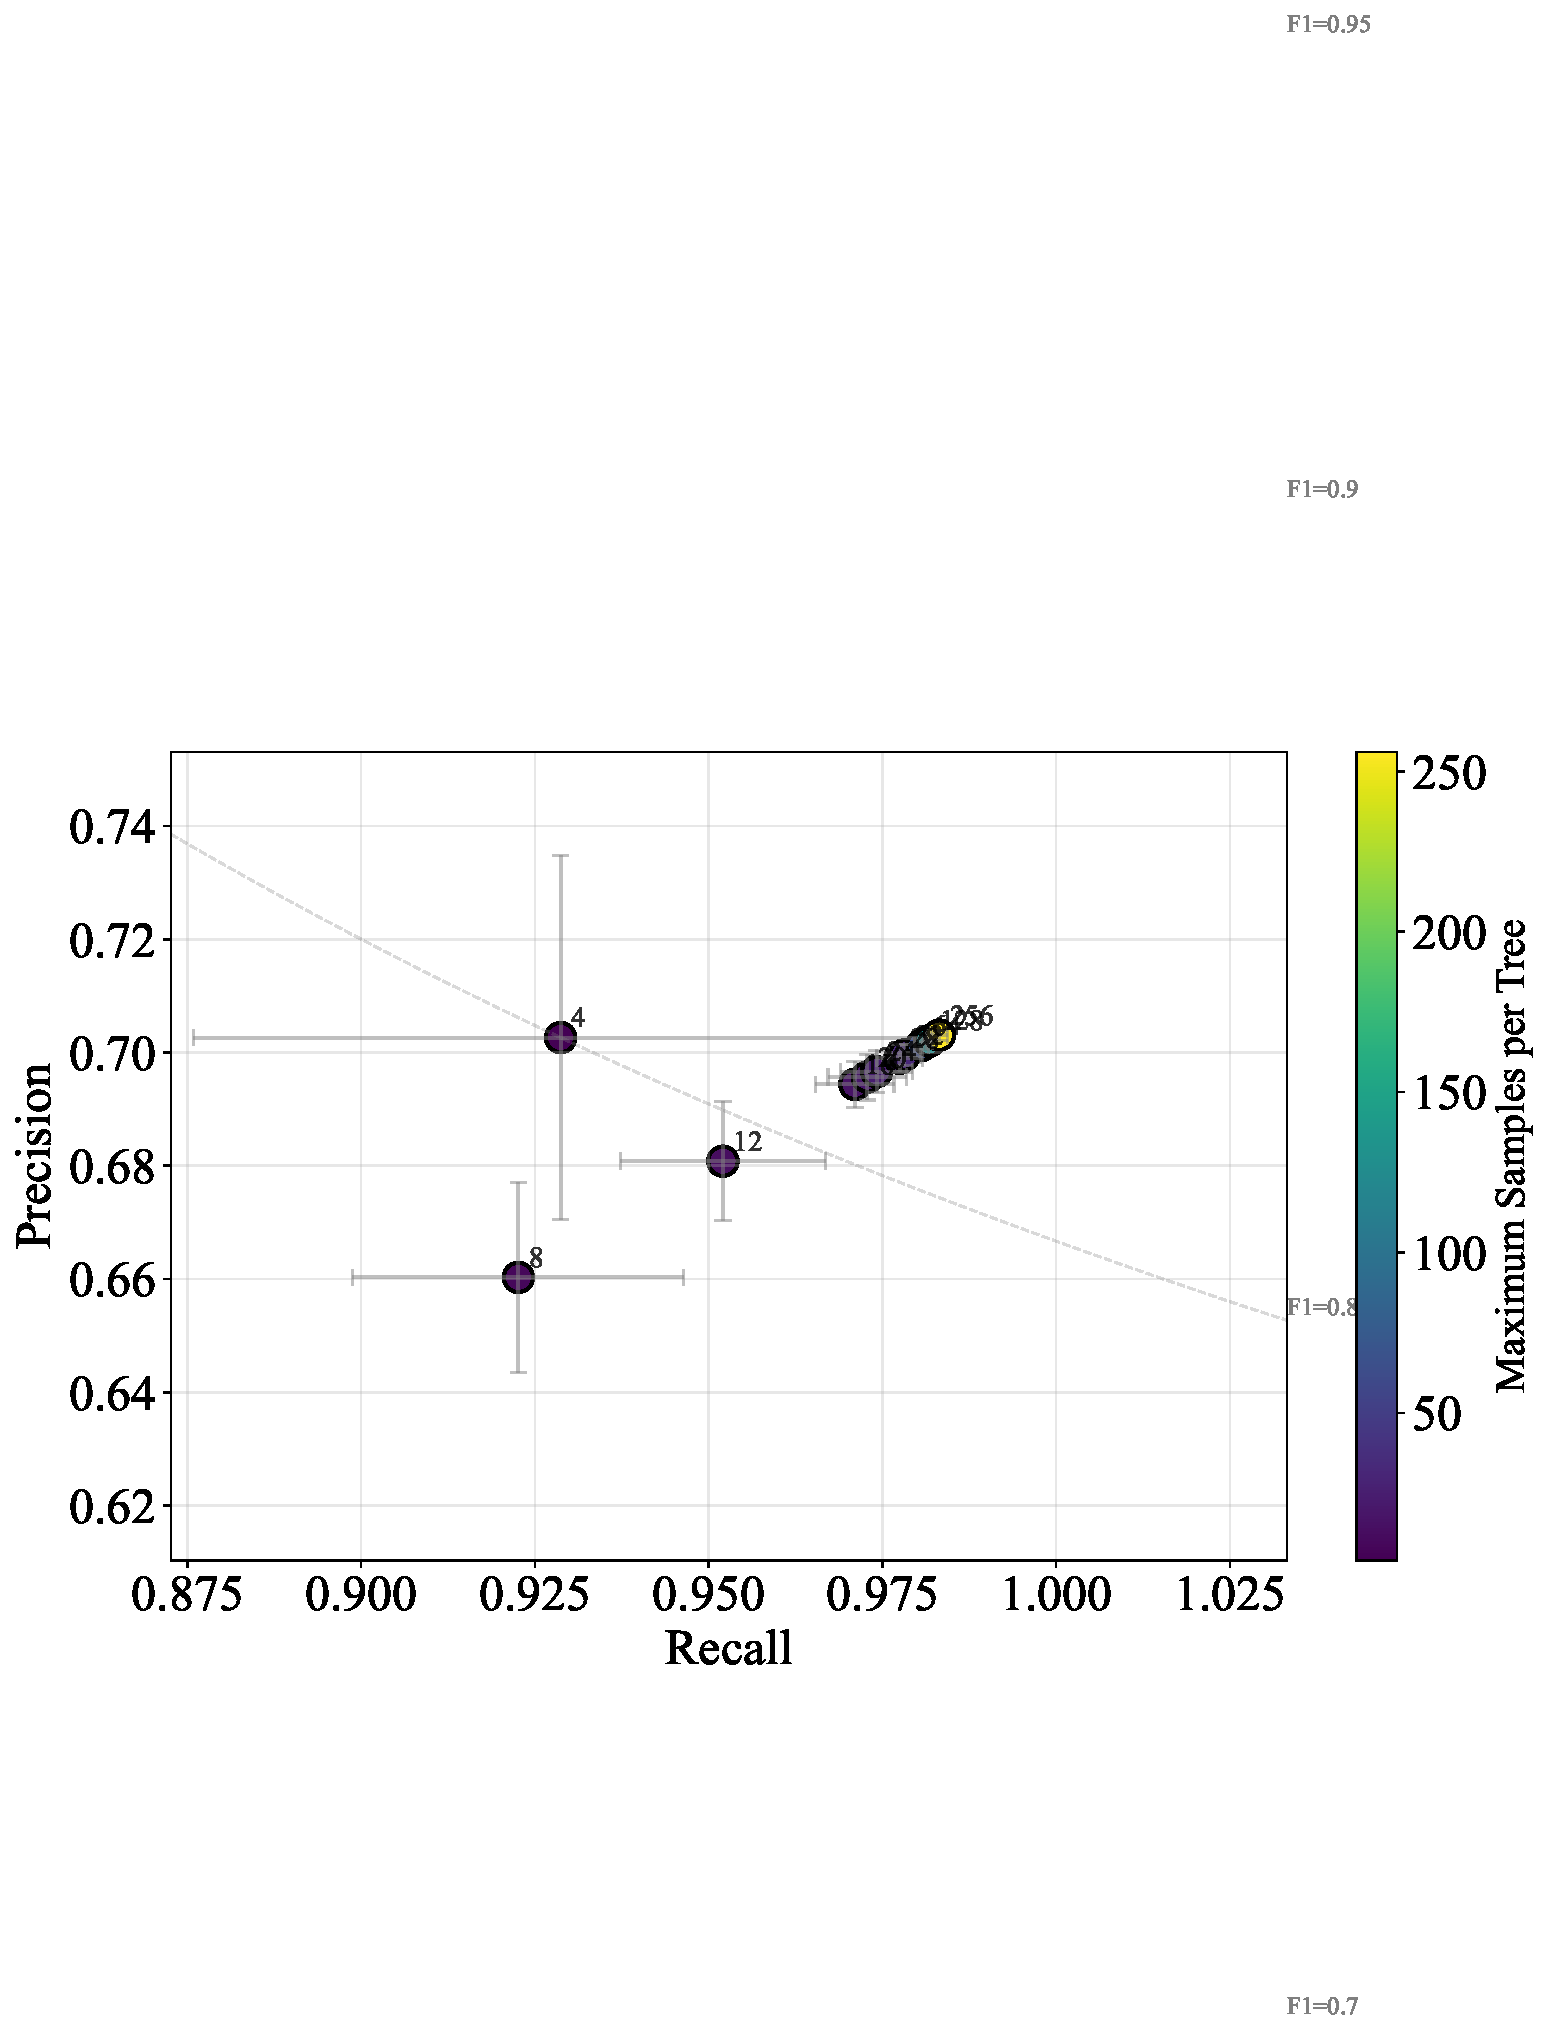
\includegraphics[width=\linewidth]{../results/shuttle/max_samples/precision_recall_tradeoff.pdf}
	\caption{Precision recall trade-off for shuttle dataset for various maximum sample parameters.}
	\label{fig:max_samples_shuttle}
\end{figure}


\subsubsection{Training Time Complexity}
% fig
% is siblinear?
% comp advatnages?
The slope of the training time against maximum samples curve for the campaign dataset was 0.072, which indicates that training time increases very slowly with sample size, confirming the Isolation Forest’s sublinear computational complexity ($O(n^{0.07})$), where runtime grows far slower than the number of samples. The knee of the curve is where the maximum samples parameter is 12 marks the point of diminishing returns, beyond which training time continues to rise while F1-score improvements plateau around 0.2365. A similar trend was observed in the shuttle dataset in Figure~\ref{fig:tt_samples_shuttle}. Unlike the campaign and shuttle datasets, where training time increased slightly with sample size, the negative slope in the fraud dataset (–0.097) indicates that for this dataset, larger subsamples actually led to more slightly more efficient training. This is illustrated in Figure~\ref{fig:tt_samples_fraud} possibly due to reduced variance in tree construction. The performance peaked later at a maximum samples parameter of 64, reflecting a higher data complexity.
 
\begin{figure}[H]
	\centering
	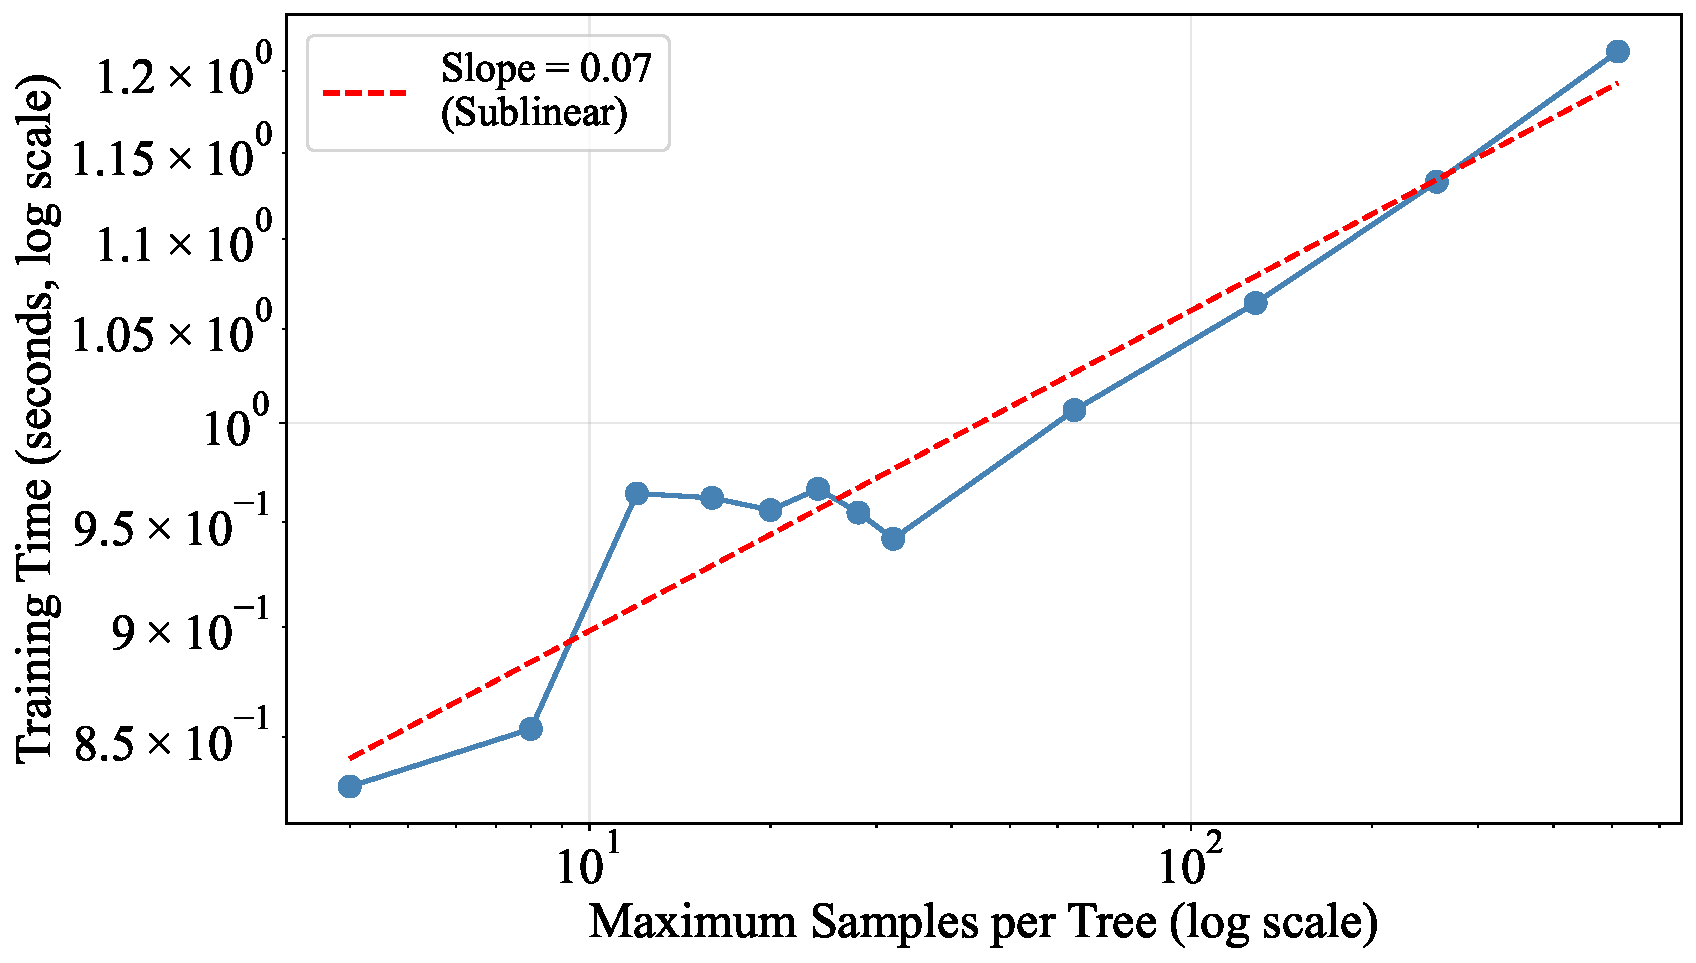
\includegraphics[width=0.95\linewidth]{../results/campaign/max_samples/training_time_scaling.pdf}
	\caption{Training time scaling with maximum samples parameter for campaign dataset.}
	\label{fig:tt_samples_campaign}
\end{figure}

Based on these findings, if computational efficiency is paramount, practitioners should set the maximum samples parameter at the knee of the curve (around 12-64 depending on dataset complexity) to balance training efficiency with model performance. Exceeding this point yields diminishing returns in F1-score improvement while unnecessarily increasing computational cost.


\subsubsection{Empirical Rule Derivation}
% fig
The best performing rule was to use $\texttt{max\_samples}=\sqrt{n}$, where $n$ is the number of observations in the dataset. This rule recommended values that produced the largest F1-score for each dataset, observed in Figure~\ref{fig:rule_samples_shuttle}, Figure~\ref{fig:rule_samples_campaign} and Figure~\ref{fig:rule_samples_fraud}. Notably, this rule ($\sqrt{284807}=533$) produced a better F1-score than simply using a fixed value of 256 for the larger fraud dataset. That is, 0.2747 as opposed to 0.2637. Therefore, it can be concluded that for larger datasets, a larger maximum sample parameter value should be considered.
\begin{figure}[H]
	\centering
	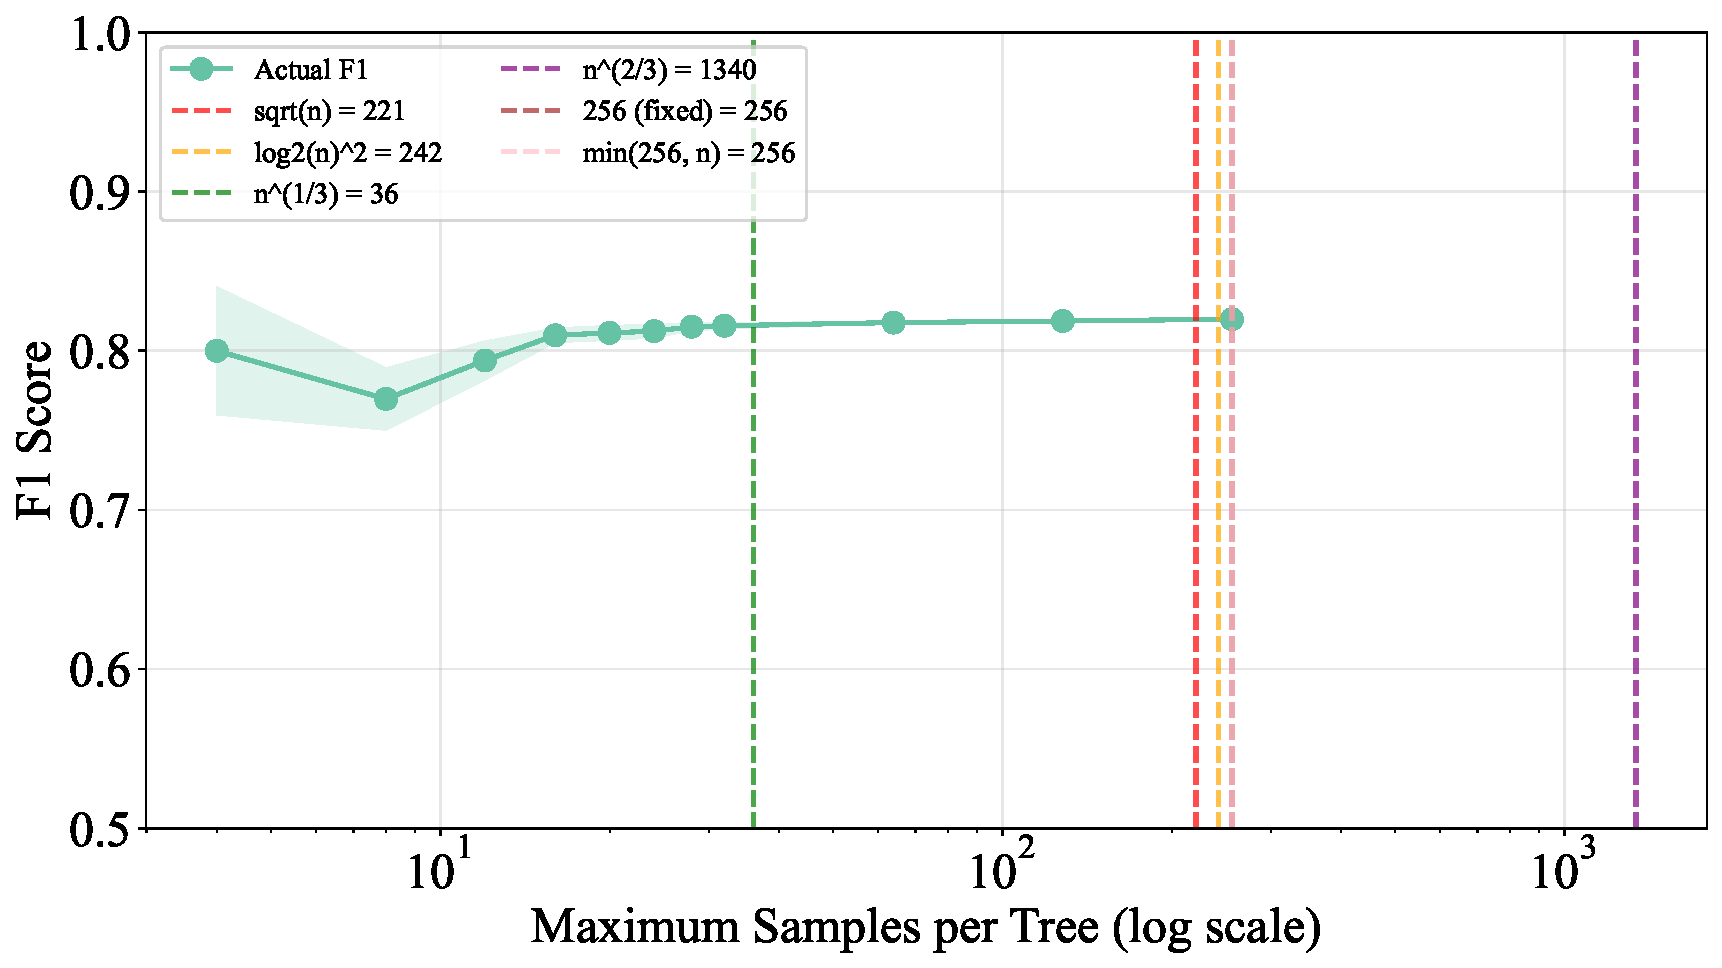
\includegraphics[width=0.95\linewidth]{../results/shuttle/max_samples/empirical_rules.pdf}
	\caption{F1-score for various maximum samples parameter rules for shuttle dataset.}
	\label{fig:rule_samples_shuttle}
\end{figure}



\subsection{Contamination Parameter}
\subsubsection{Robustness to Misspecification}
% fig: perfromance - heatmap or line plot
Since this parameter is directly used by the algorithm to determine the threshold at which to classify an observation as an anomaly, the F1-score peaks at the contamination value that matches the correct percentage of anomalies in the dataset. For example, in Figure~\ref{fig:contamination_all} the F1-score is greatest for the shuttle dataset at approximately 0.0715 which matches the anomaly rate of the dataset of 7.15\%. It is important to consider this parameter carefully, as it is not robust to misspecification.
\begin{figure}[H]
	\centering
	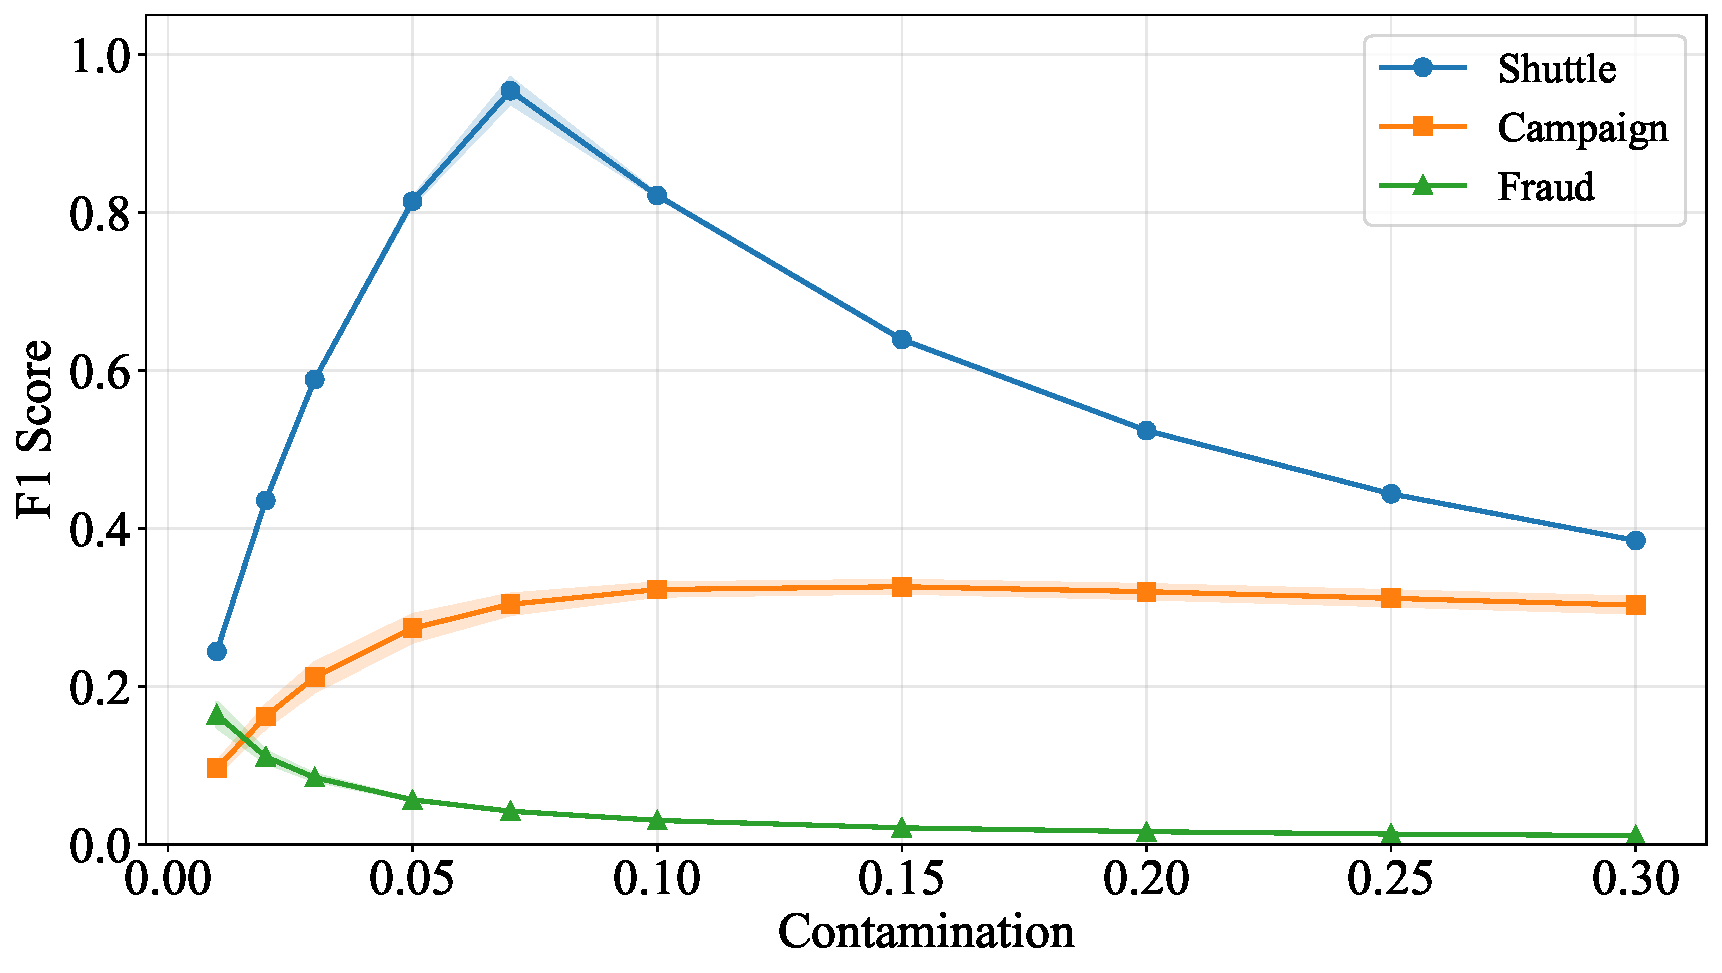
\includegraphics[width=0.95\linewidth]{../results/multi_dataset/contamination_f1.pdf}
	\caption{Performance with increasing values of the contamination parameter.}
	\label{fig:contamination_all}
\end{figure}
% over or under

% why IF robust to errors?

% practical overestinamation?  - some cases want overestimate like fraud


Underestimating contamination severely degraded performance in the campaign dataset (average F1: 0.2281) compared to overestimating (average F1: 0.3150), with underestimation performing 8.69\% worse. This indicates it is safer to overestimate the contamination rate when the true anomaly proportion is uncertain. The plot in Figure~\ref{fig:contamination_campaign} describes this trend. A similar trend was observed in the shuttle dataset seen in Figure~\ref{fig:contamination_shuttle}.

\begin{figure}[H]
	\centering
	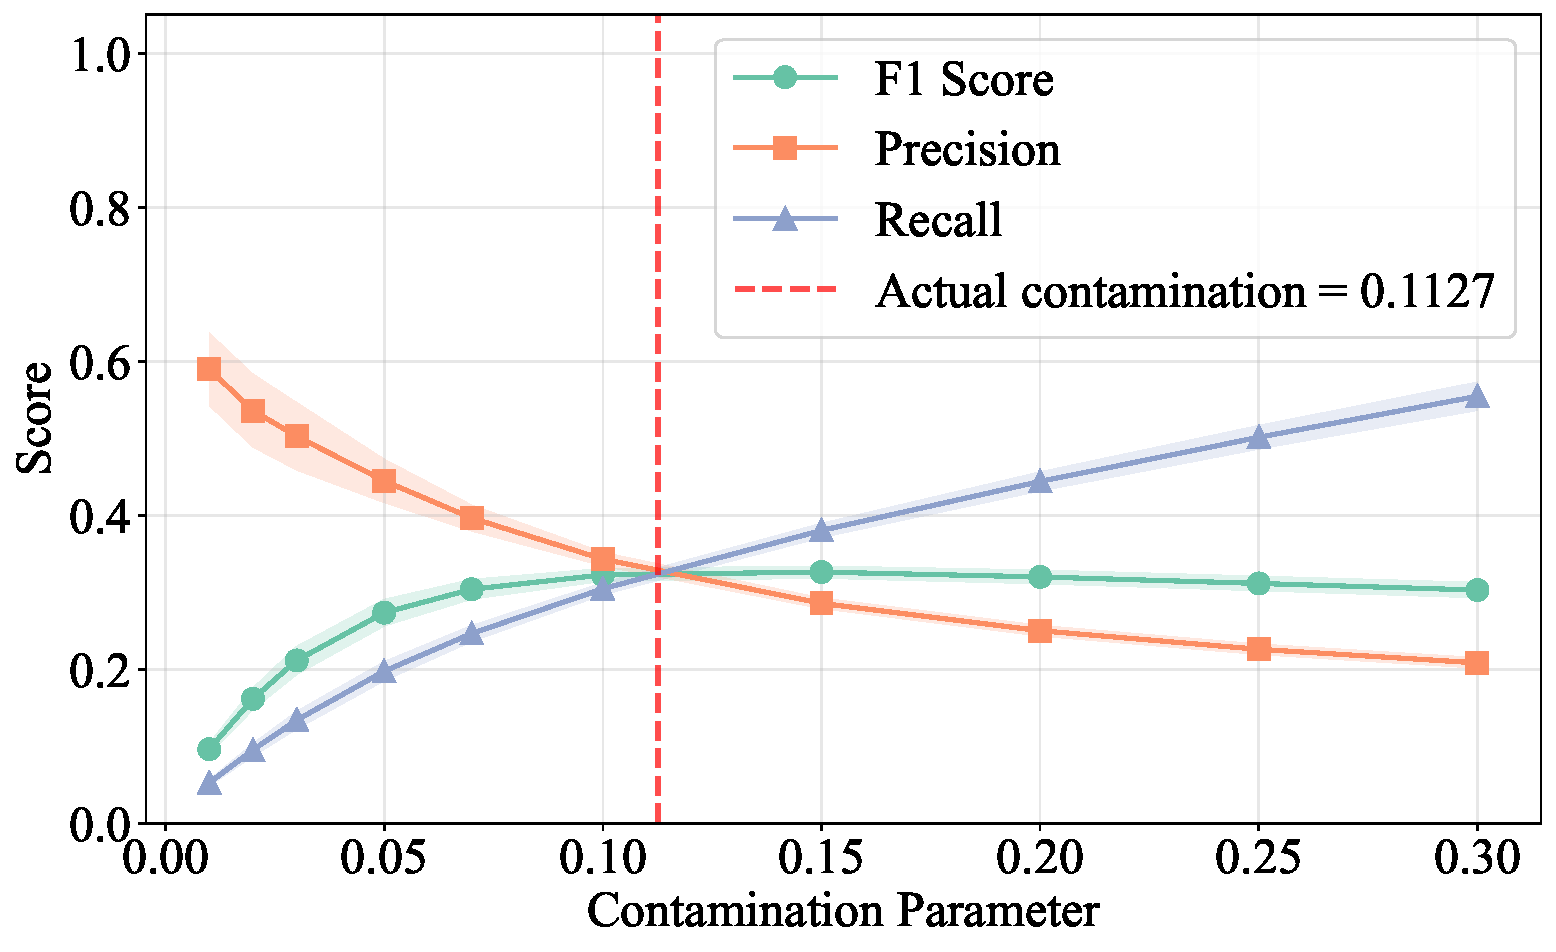
\includegraphics[width=0.95\linewidth]{../results/campaign/contamination/performance_vs_contamination.pdf}
	\caption{Performance with increasing values of the contamination parameter for campaign dataset.}
	\label{fig:contamination_campaign}
\end{figure}


\subsubsection{Calibration Analysis}
% idk have a closer look
Since the algorithm directly controls the number of predicted anomalies with the contamination parameter, the calibration error was near 0 for all parameter values. This is shown in Figure~\ref{fig:contamination_shuttle_calibration}.
\begin{figure}[H]
	\centering
	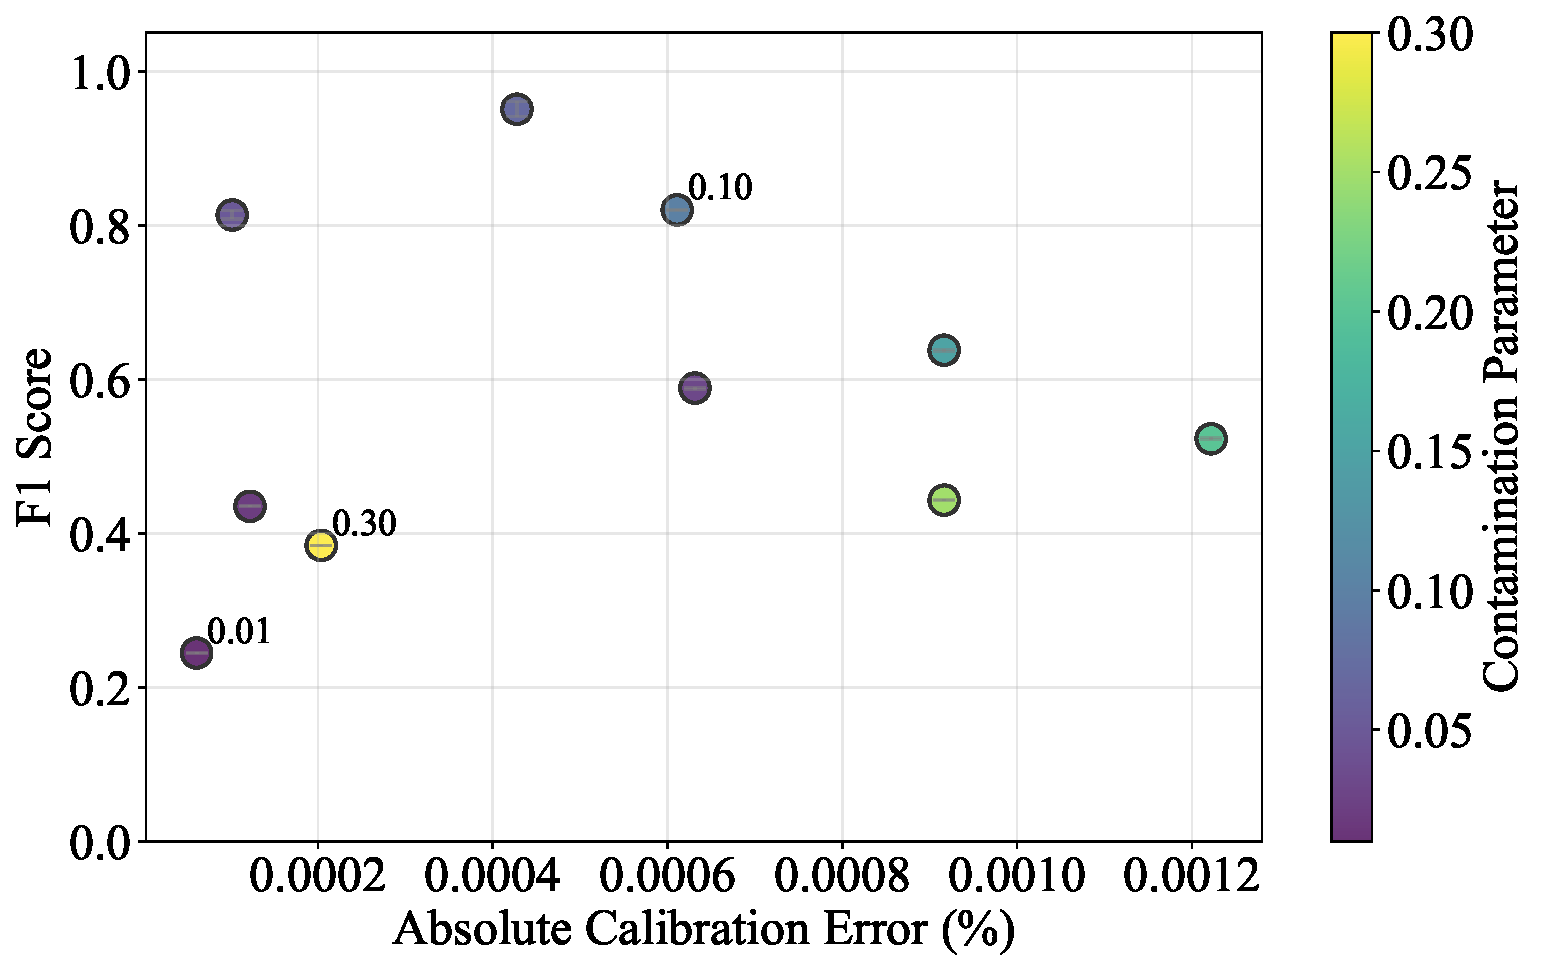
\includegraphics[width=0.95\linewidth]{../results/shuttle/contamination/f1_vs_calibration_error.pdf}
	\caption{Calibration errors for various contamination values.}
	\label{fig:contamination_shuttle_calibration}
\end{figure}

\subsection{Maximum Features}
\subsubsection{Performance}
% fig: f1 ... vs max featu
% observe high dim improve
% low dim degredation?
% curse of dimensionality miitgation
% irrelevant feature noise reduction
% when full features are necessary

For the shuttle dataset, considering all 9 features led to the best performance as shown in Figure~\ref{fig:max_features_shuttle}. Interestingly, only one feature per split produced surprisingly good performance, and two features brought the performance to near optimal. For the campaign dataset on the other hand, fewer features per split resulted in slightly better performance as illustrated in Figure~\ref{fig:max_features_campaign}. The fraud dataset reported the highest F1-score with the maximum features parameter at one, seen in Figure~\ref{fig:max_features_fraud}.

These contrasting results highlight the importance of dataset-specific tuning for the maximum features control parameter. Low-dimensional datasets with few features (like shuttle) benefit from considering more (or all) features per split to capture complex decision boundaries, while datasets with noisy or redundant features (like campaign and fraud) may achieve better generalisation by limiting feature consideration and reducing overfitting.


\begin{figure}[H]
	\centering
	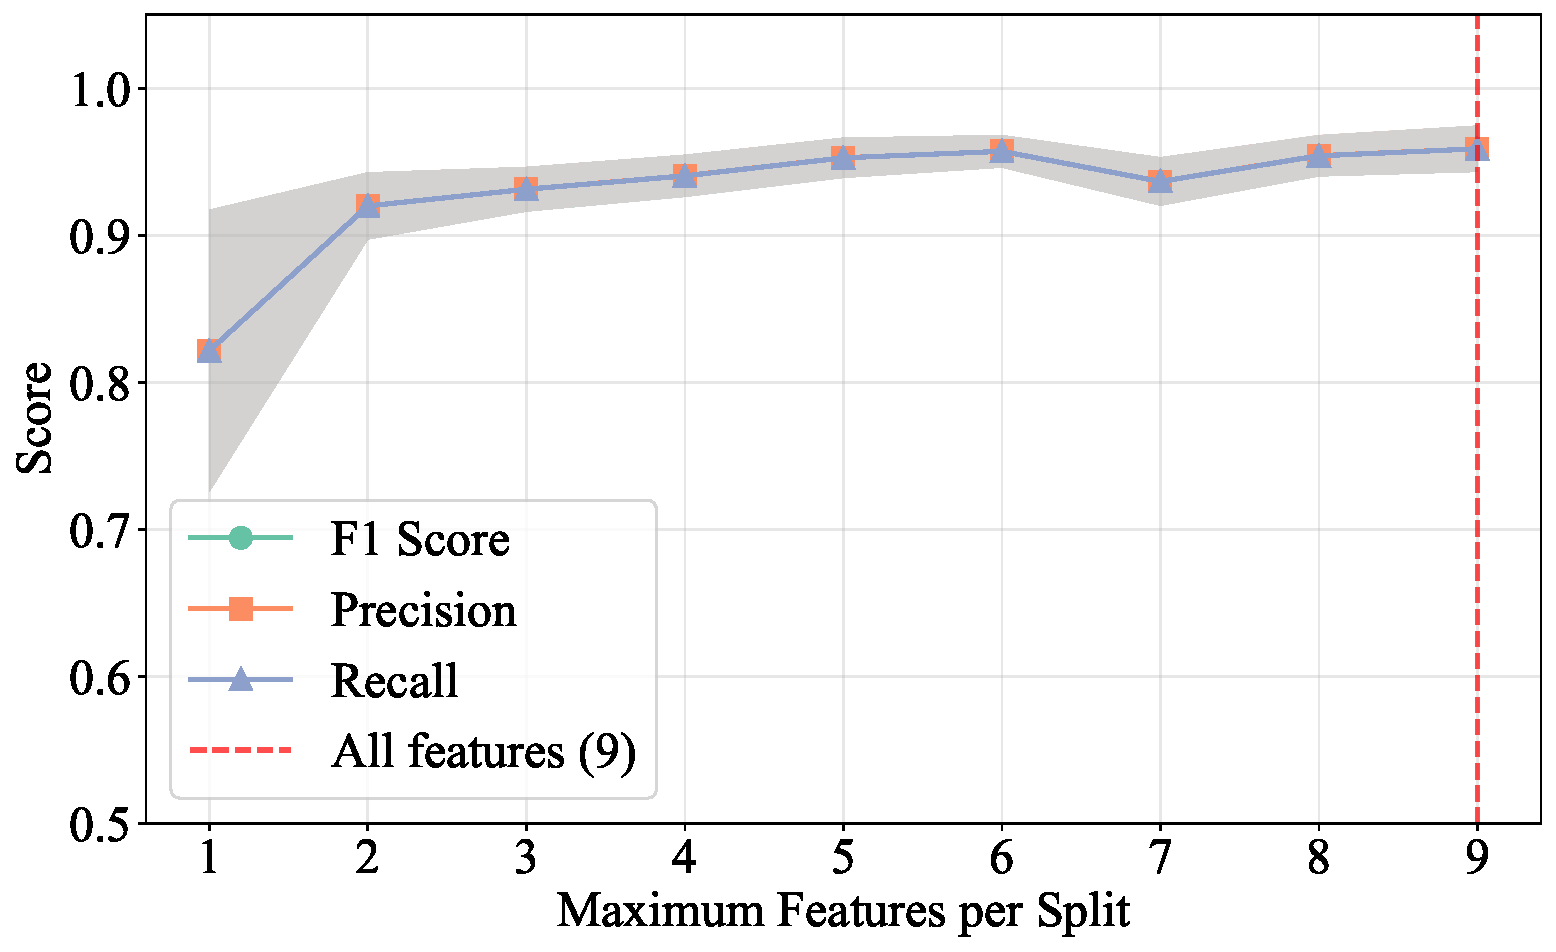
\includegraphics[width=0.95\linewidth]{../results/shuttle/max_features/performance_vs_max_features.pdf}
	\caption{Performance of maximum features parameter for shuttle dataset.}
	\label{fig:max_features_shuttle}
\end{figure}

\subsubsection{Efficiency-Performance Trade-off}
% fig: dual axis plot f1 and time v max feat

% observe sweet spot and data specific patterns
% give practical recommendation for high dim data, mention diminishing returns
The efficiency of the maximum features parameter tended to decreases as more features were considered per split for the campaign and fraud datasets. This is shown in Figure~\ref{fig:max_features_tt_campaign}. This aligns with the diminishing returns explained in the previous section, as the majority of the anomalies could be found by considering only a few features for a split. On the other hand, the shuttle dataset showed increased efficiency as more features were considered, illustrated in Figure~\ref{fig:max_features_tt_shuttle}. This contrast suggests that the optimal number of features per split is highly dataset-dependent, influenced by the underlying feature relevance and redundancy.




\begin{figure}[H]
	\centering
	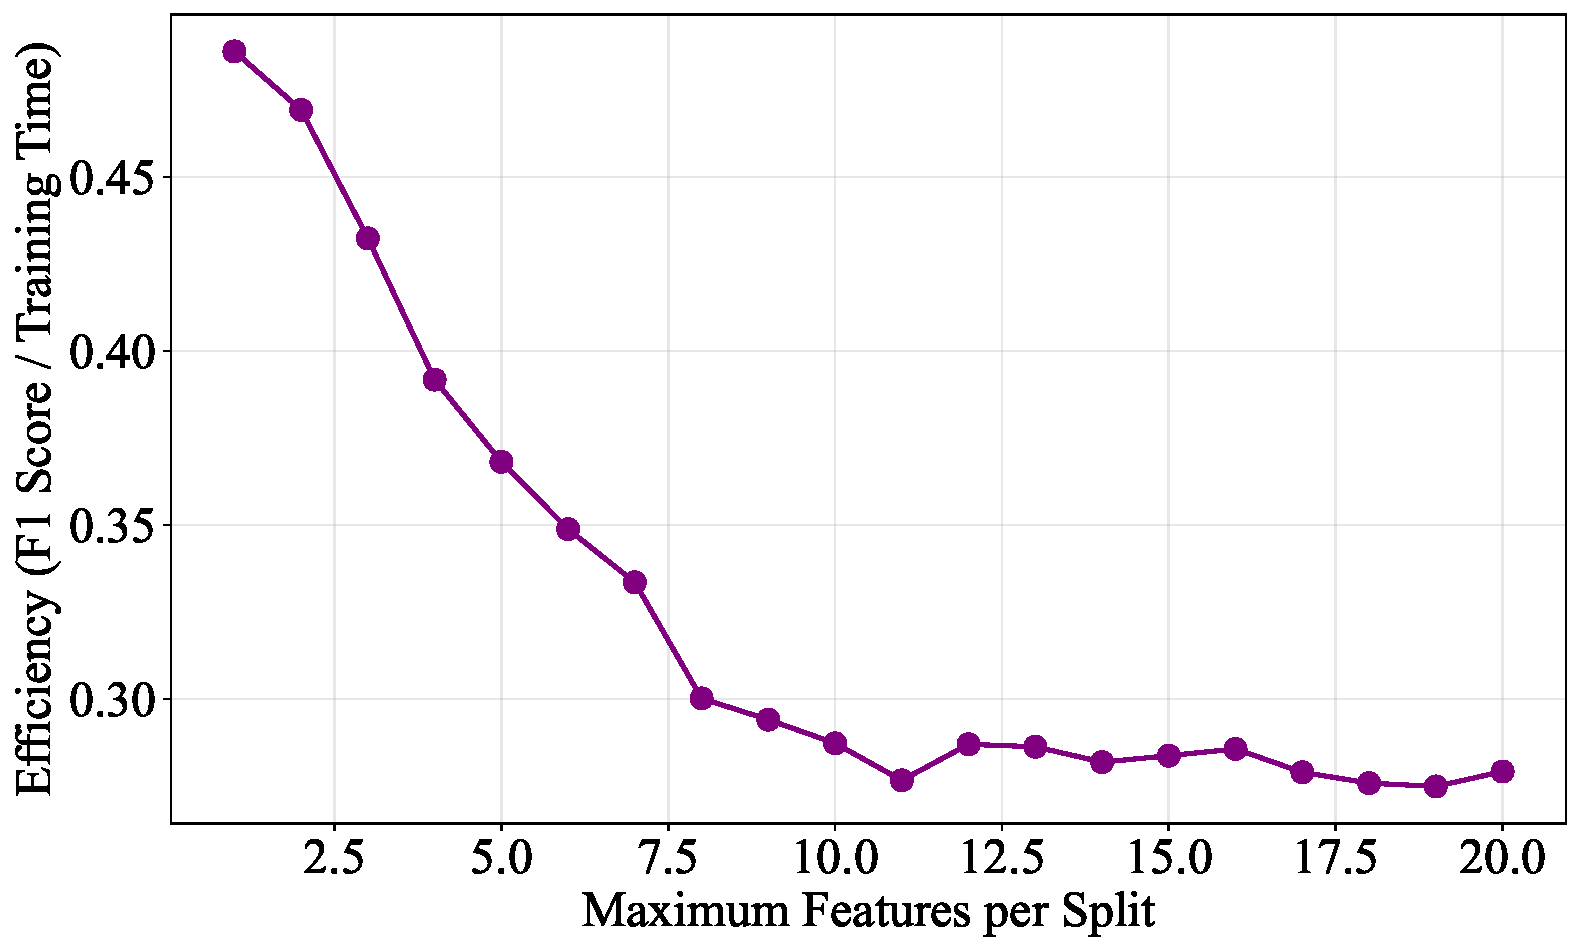
\includegraphics[width=0.95\linewidth]{../results/campaign/max_features/efficiency_vs_max_features.pdf}
	\caption{Training time of maximum features parameter for campaign dataset.}
	\label{fig:max_features_tt_campaign}
\end{figure}

\subsubsection{Interaction with Ensemble Size}
% fig: speech only heatmap of f1 score
% obseve can more trees compensate for fewer features?
% trade ioff
% practical guidance
The model performance benefited from both an increase in the number of estimators and the number of features considered per split, shown in Figure~\ref{fig:int_hm_shuttle}.  On the other hand, the number of estimators increased the training time significantly more than the number of features. This is seen in Figure~\ref{fig:int_hm_tt_shuttle}. The campaign dataset exhibited a different trend, with still more estimators favourable, but fewer features considered. This is shown in Figure~\ref{fig:int_hm_campaign}. The fraud dataset was least affected by the maximum features parameter, shown in Figure~\ref{fig:int_3d_fraud}.




\begin{figure}[H]
	\centering
	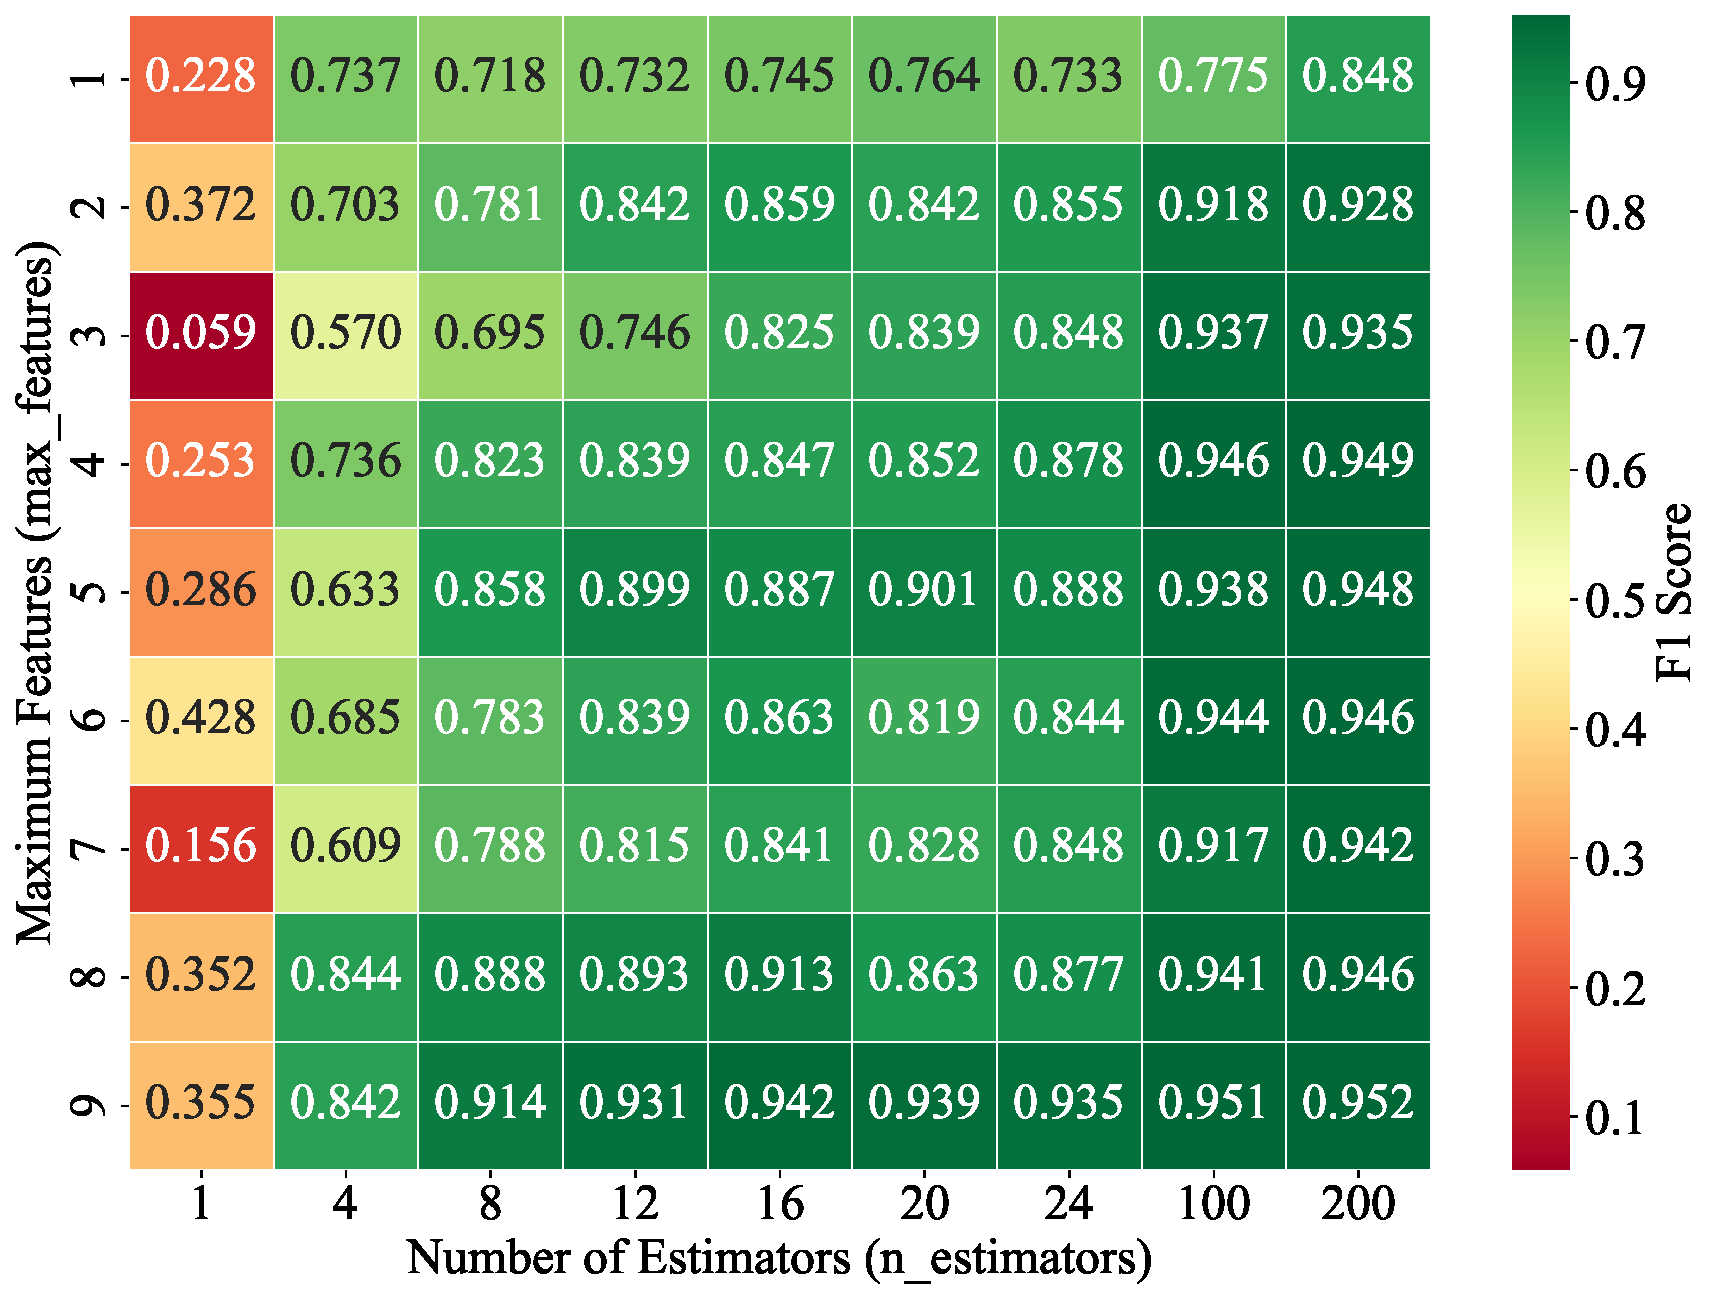
\includegraphics[width=0.95\linewidth]{../results/shuttle/max_features/interaction_f1_heatmap.pdf}
	\caption{Interaction heatmap for number of features and estimators for shuttle dataset.}
	\label{fig:int_hm_shuttle}
\end{figure}


\begin{figure}[H]
	\centering
	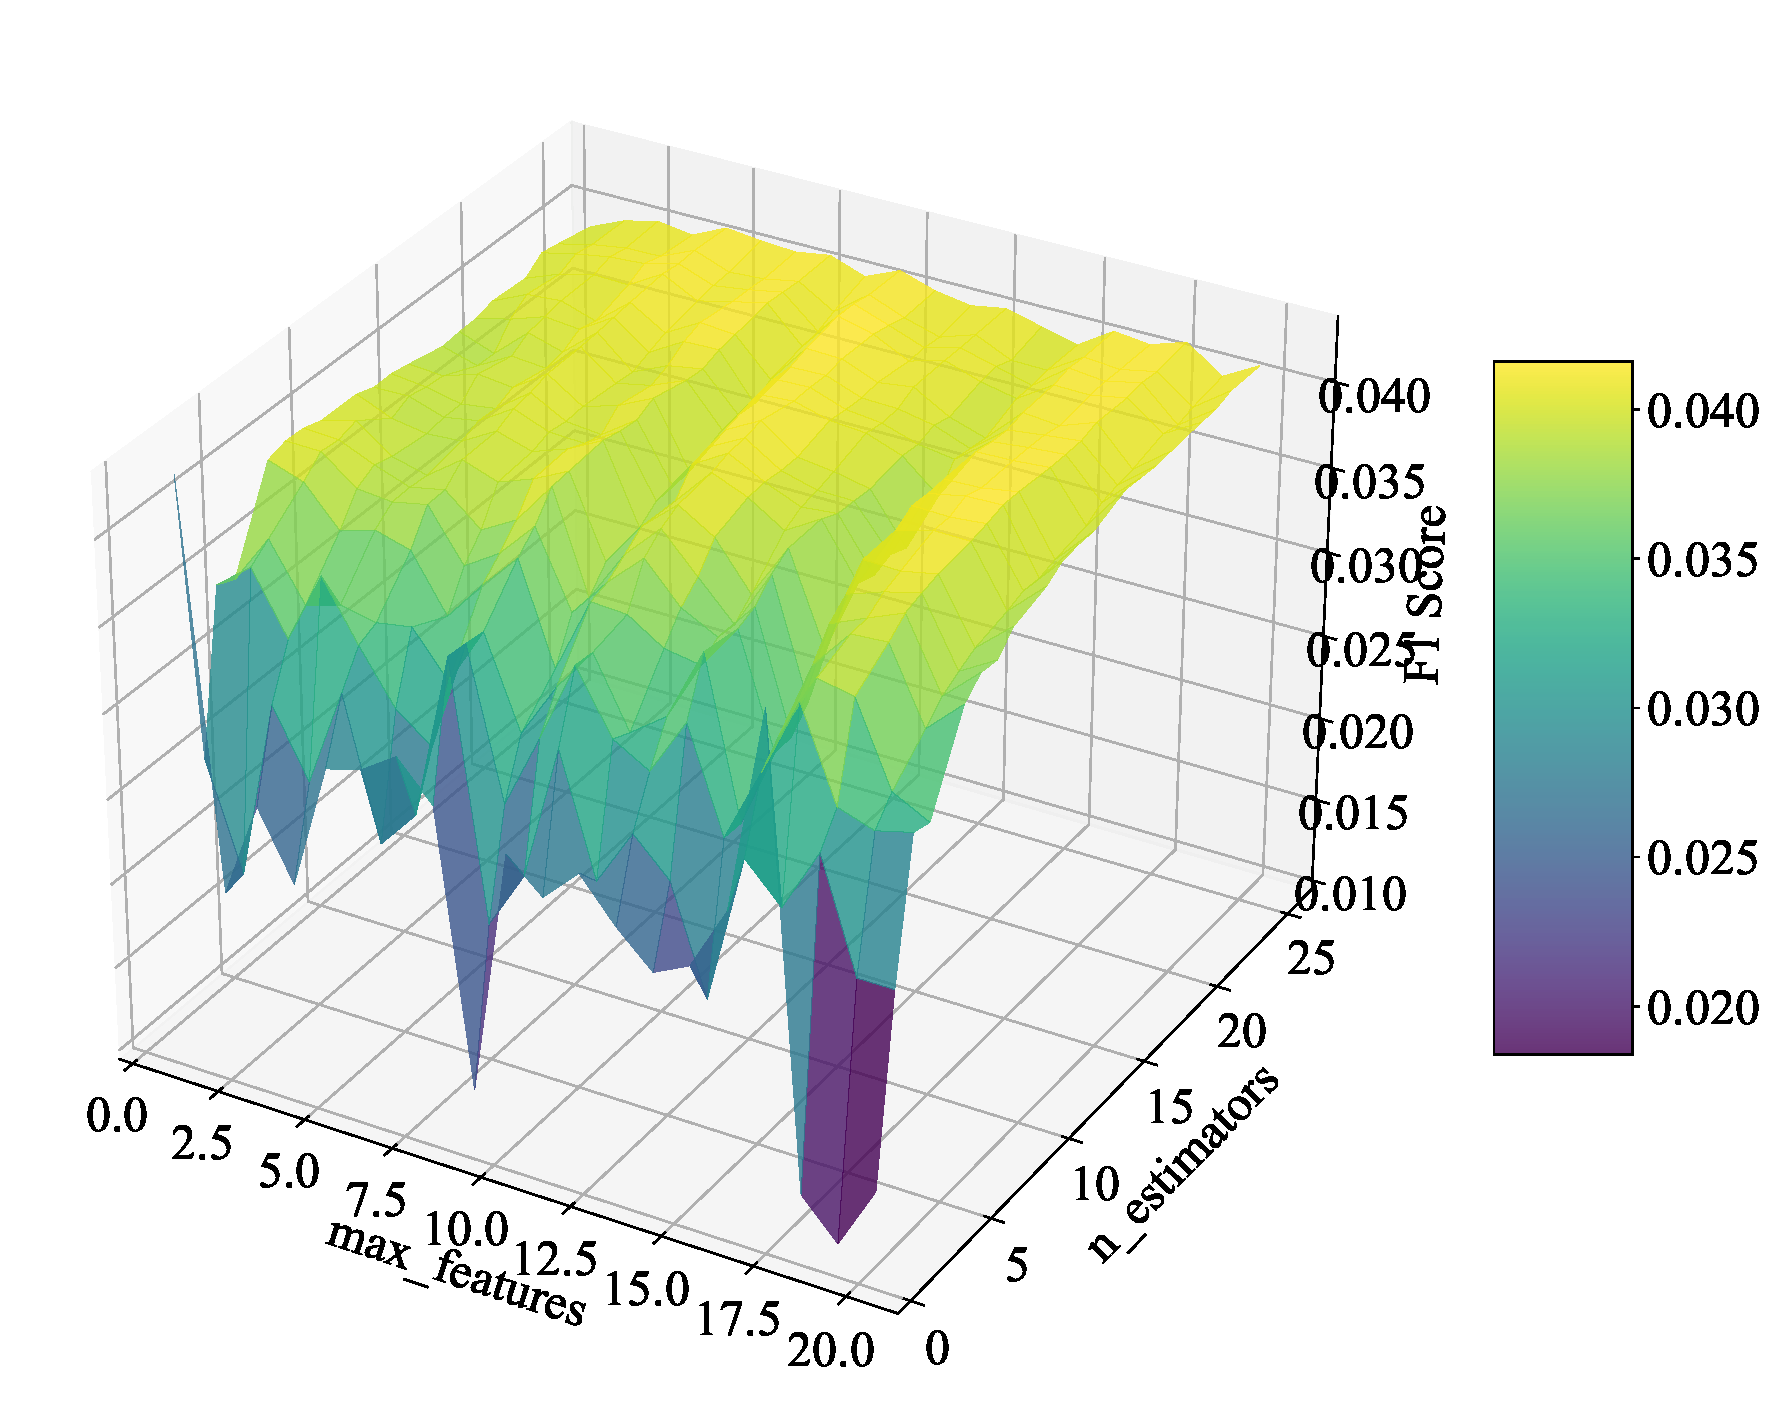
\includegraphics[width=0.95\linewidth]{../results/fraud/max_features/interaction_3d_surface.pdf}
	\caption{Interaction plot for number of features, estimators and F1-score for fraud dataset.}
	\label{fig:int_3d_fraud}
\end{figure}

Critically, the analysis revealed that ensemble size cannot effectively compensate for insufficient feature availability, configurations with limited features but many estimators consistently underperformed compared to configurations with adequate features and fewer estimators. Restricting features created a performance ceiling that additional trees cannot overcome.


\subsection{Bootstrap Parameter}
\subsubsection{Stability Comparison}
% fig: box plots with and without bootstrap

% statistical wilcoxon signed rank
% effect size cohen's d annotation
% variance differences across datasets
% statistical sig
The Cohen's d values for all the datasets were below 0.1, meaning that the bootstrap parameter had a negligible effect. The boxplots in Figure~\ref{fig:bootstrap_shuttle}, Figure~\ref{fig:bootstrap_campaign}, and Figure~\ref{fig:bootstrap_fraud} show that the bootstrap parameter can sometimes slightly decrease the performance of the isolation tree model. The performance did remain stable for both parameter options.

\begin{figure}[H]
	\centering
	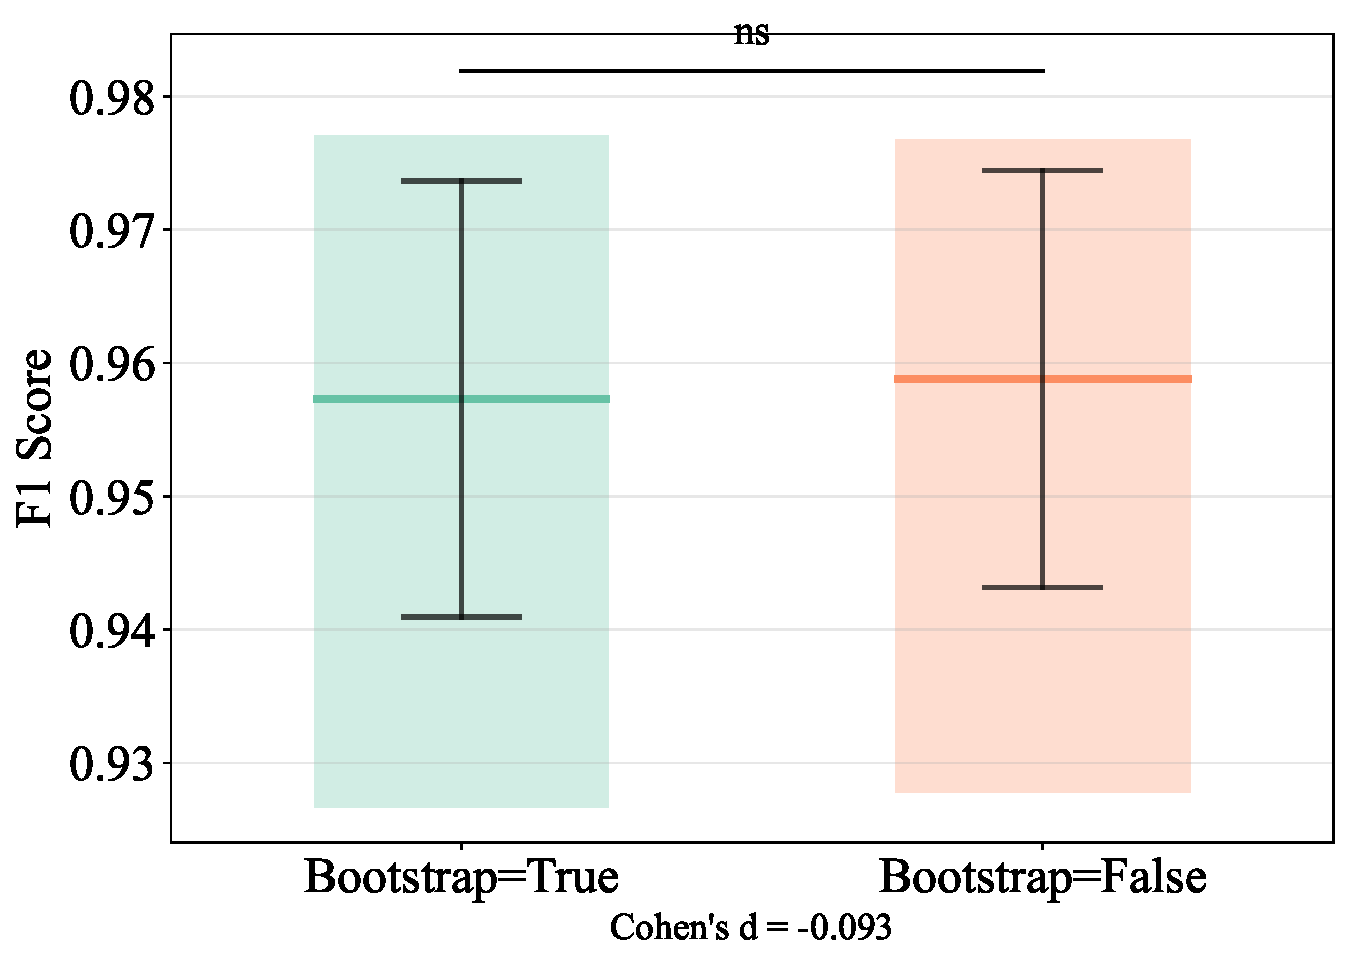
\includegraphics[width=0.95\linewidth]{../results/shuttle/bootstrap/bootstrap_stability_box.pdf}
	\caption{Bootstrap stability for shuttle dataset.}
	\label{fig:bootstrap_shuttle}
\end{figure}

\subsubsection{Performance Metrics}
% give table of performance
The performance only slightly increased using the bootstrap parameter for the fraud dataset where the F1-score  increase by 0.196\%, seen in Table~\ref{tab:bootstrap_comparison}. The datasets consulted in this paper revealed that the bootstrap parameter can be safely ignored for most anomaly detection problems, as it provides little to no improvement in model performance.
\begin{table}[htbp]
	\caption{Comparison of F1 Scores With and Without Bootstrapping}
	\centering
	\begin{tabular}{|l|c|c|c|c|}
		\hline
		\textbf{Dataset} & \textbf{Bootstrap=T} & \textbf{Bootstrap=F} & \textbf{Difference} & \textbf{\% Change} \\ 
		\hline
		shuttle & 0.957305 & 0.958800 & -0.001496 & -0.156021 \\ 
		\hline
		campaign & 0.325003 & 0.325766 & -0.000763 & -0.234302 \\ 
		\hline
		fraud & 0.263675 & 0.263159 & 0.000516 & 0.196142 \\ 
		\hline
	\end{tabular}
	\label{tab:bootstrap_comparison}
\end{table}


% say how it doesnt help much

\subsubsection{Interaction with Contamination}
% fig: grouped bar

%Does bootstrap effect depend on contamination level?
The interaction between the bootstrap and contamination control parameters was explored. Experimental results from the three datasets indicated that these two variables were completely independent from each other, shown for the campaign dataset in Figure~\ref{fig:bootstrap_int_campaign}. 


\begin{figure}[H]
	\centering
	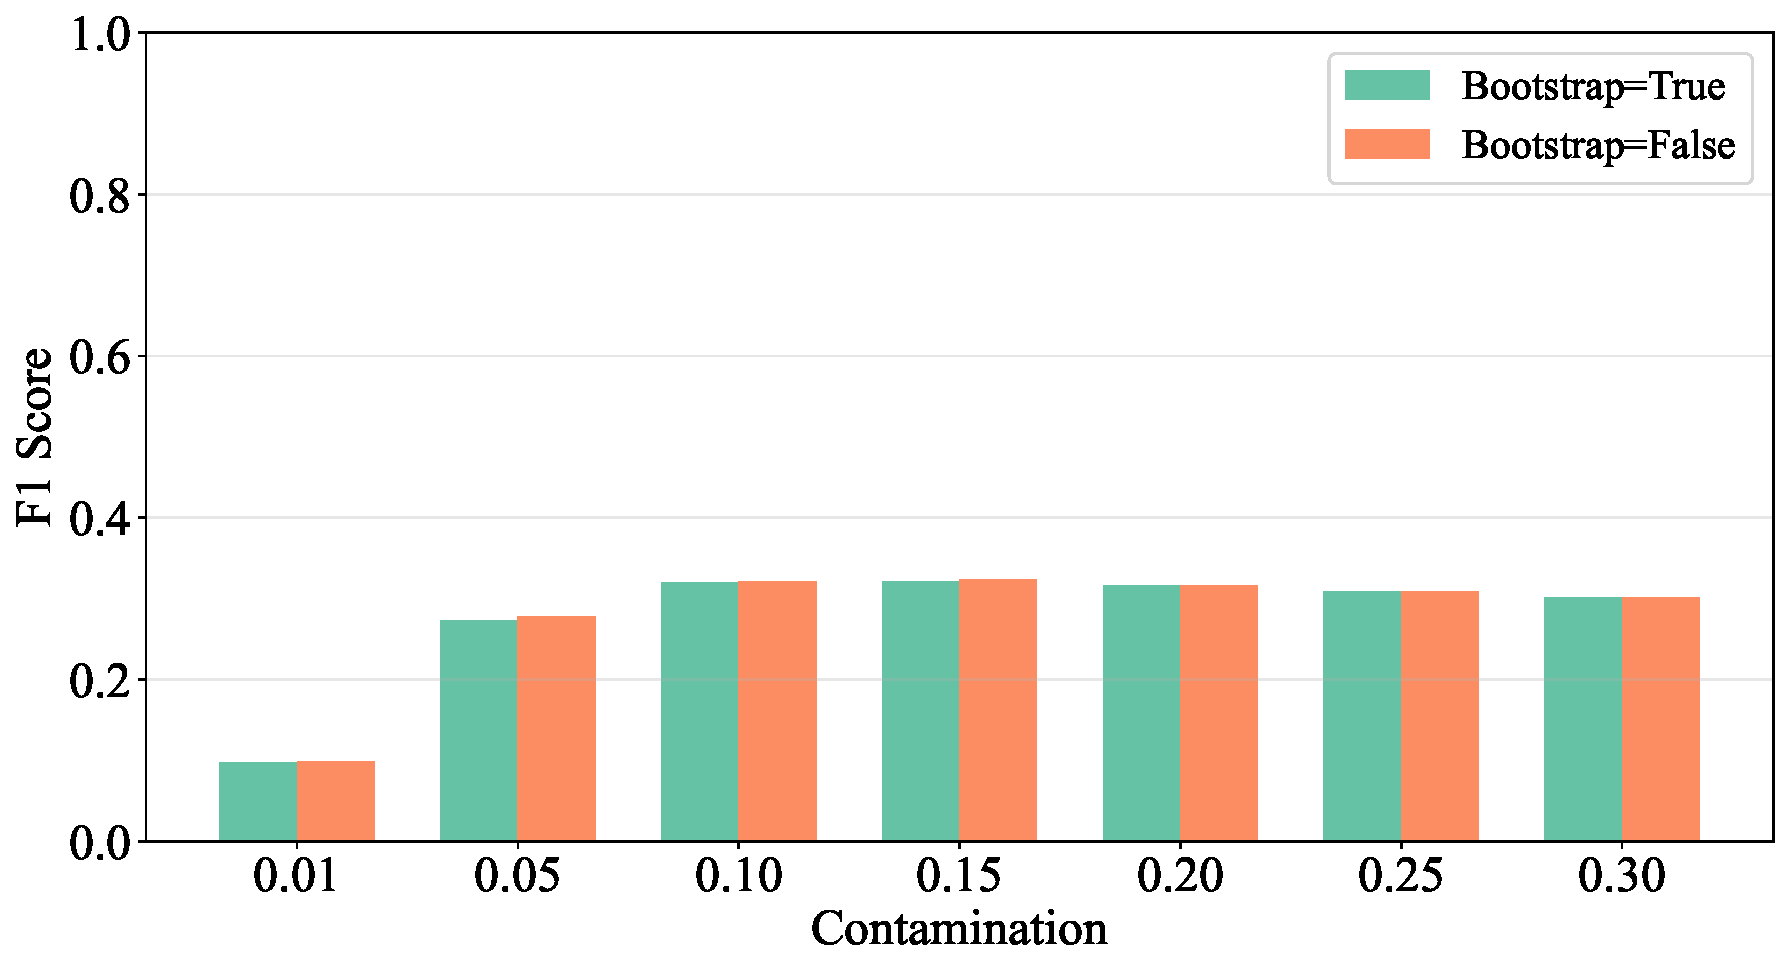
\includegraphics[width=0.95\linewidth]{../results/campaign/bootstrap/bootstrap_contamination_interaction.pdf}
	\caption{Bootstrap interaction with contamination for campaign dataset.}
	\label{fig:bootstrap_int_campaign}
\end{figure}

\subsection{Practical Guidelines}
For the majority of applications, 100-125 estimators will provide high anomaly detection ability. In resource-constrained situations, 25-50 estimators provide acceptable performance with faster training times. The rules of thumb to use $\sqrt{n}$ maximum samples outperforms the fixed value of 256 for large datasets. The swamping effect much be monitored if the F1-score drops with a larger parameter value. For best efficiency, 12-64 samples provides decent performance. The contamination parameter value should be tuned carefully since it is not robust to misspecification. For low-dimensional data, all the features should be used. However for high-dimensional data ($> 30$ features), restricting to few features reduces noise. The bootstrap parameter can be safely left disabled since it provided no real performance benefit. The only case it might be useful is for extremely small datasets where sampling variance is high.

\section{Conclusions}


\bibliographystyle{IEEEtran}
\bibliography{references}

\appendices
\section{Additional Results}
\begin{figure}[H]
	\centering
	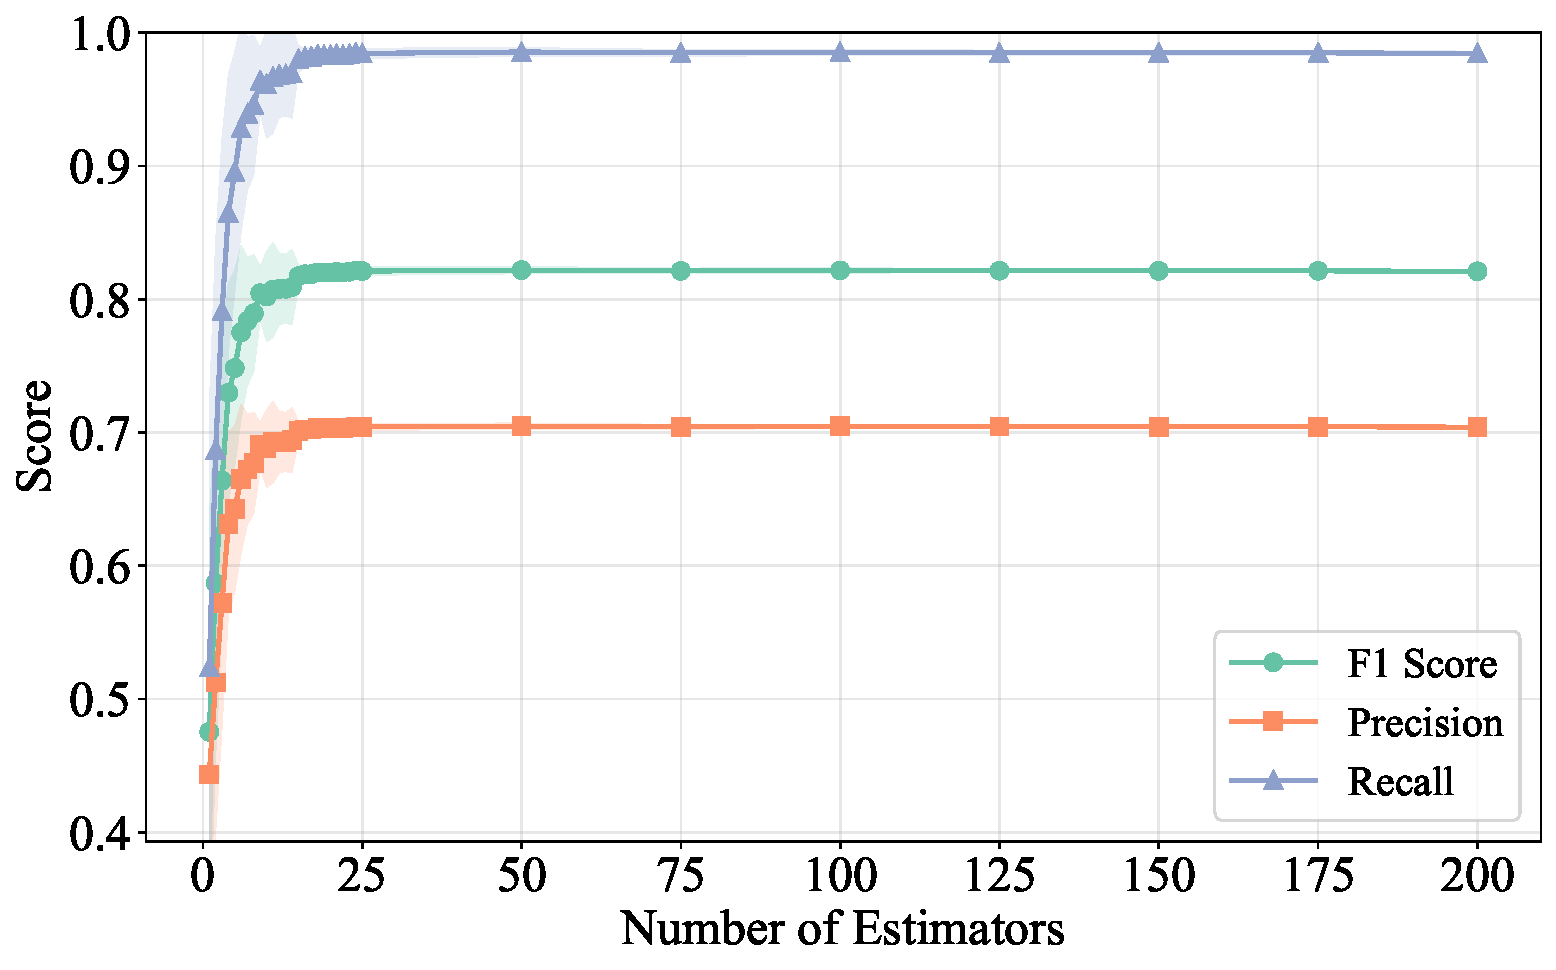
\includegraphics[width=\linewidth]{../results/shuttle/n_estimators/convergence_curve.pdf}
	\caption{Convergence curve for shuttle dataset.}
	\label{fig:n_estimators_shuttle}
\end{figure}
\begin{figure}[H]
	\centering
	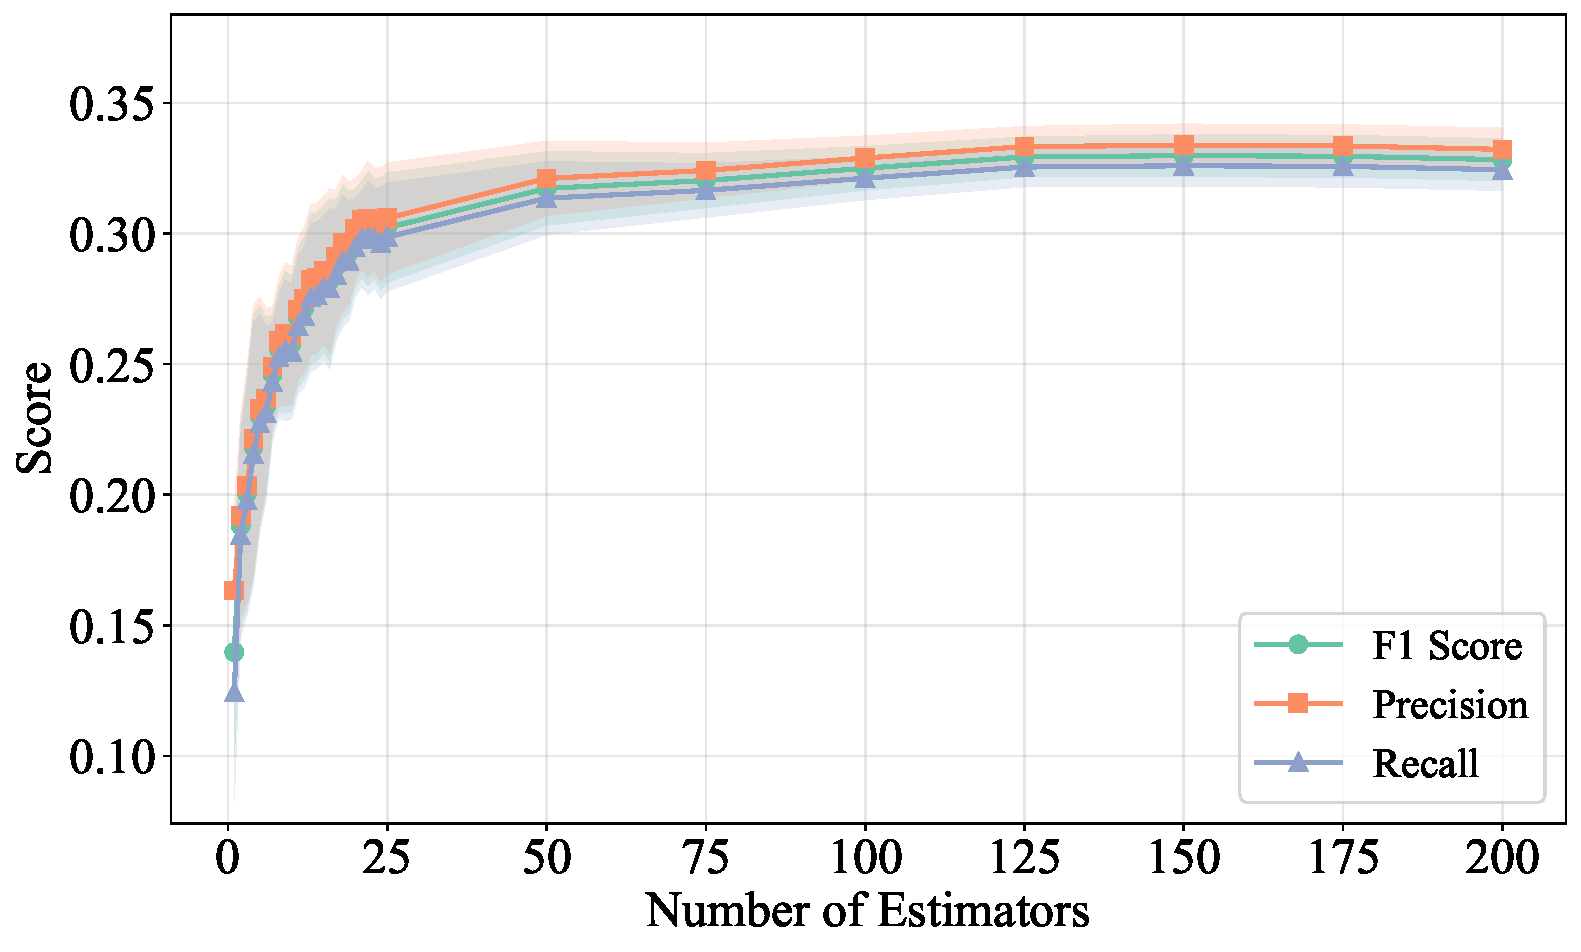
\includegraphics[width=\linewidth]{../results/campaign/n_estimators/convergence_curve.pdf}
	\caption{Convergence curve for campaign dataset.}
	\label{fig:n_estimators_campaign}
\end{figure}
\begin{figure}[H]
	\centering
	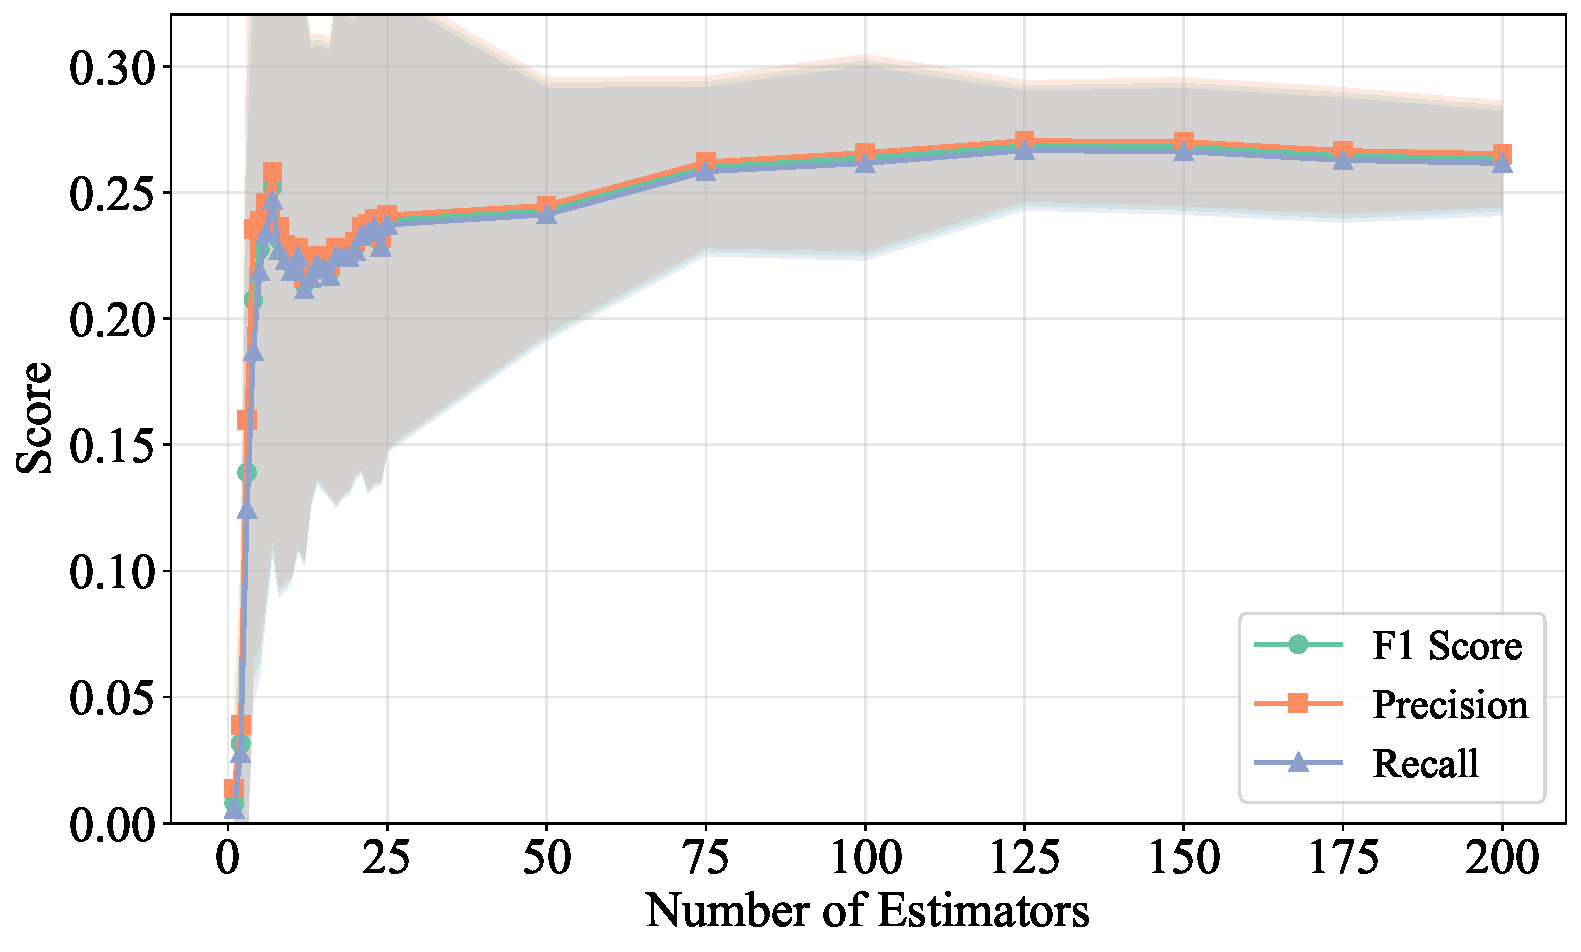
\includegraphics[width=\linewidth]{../results/fraud/n_estimators/convergence_curve.pdf}
	\caption{Convergence curve for fraud dataset.}
	\label{fig:n_estimators_fraud}
\end{figure}


\begin{figure}[H]
	\centering
	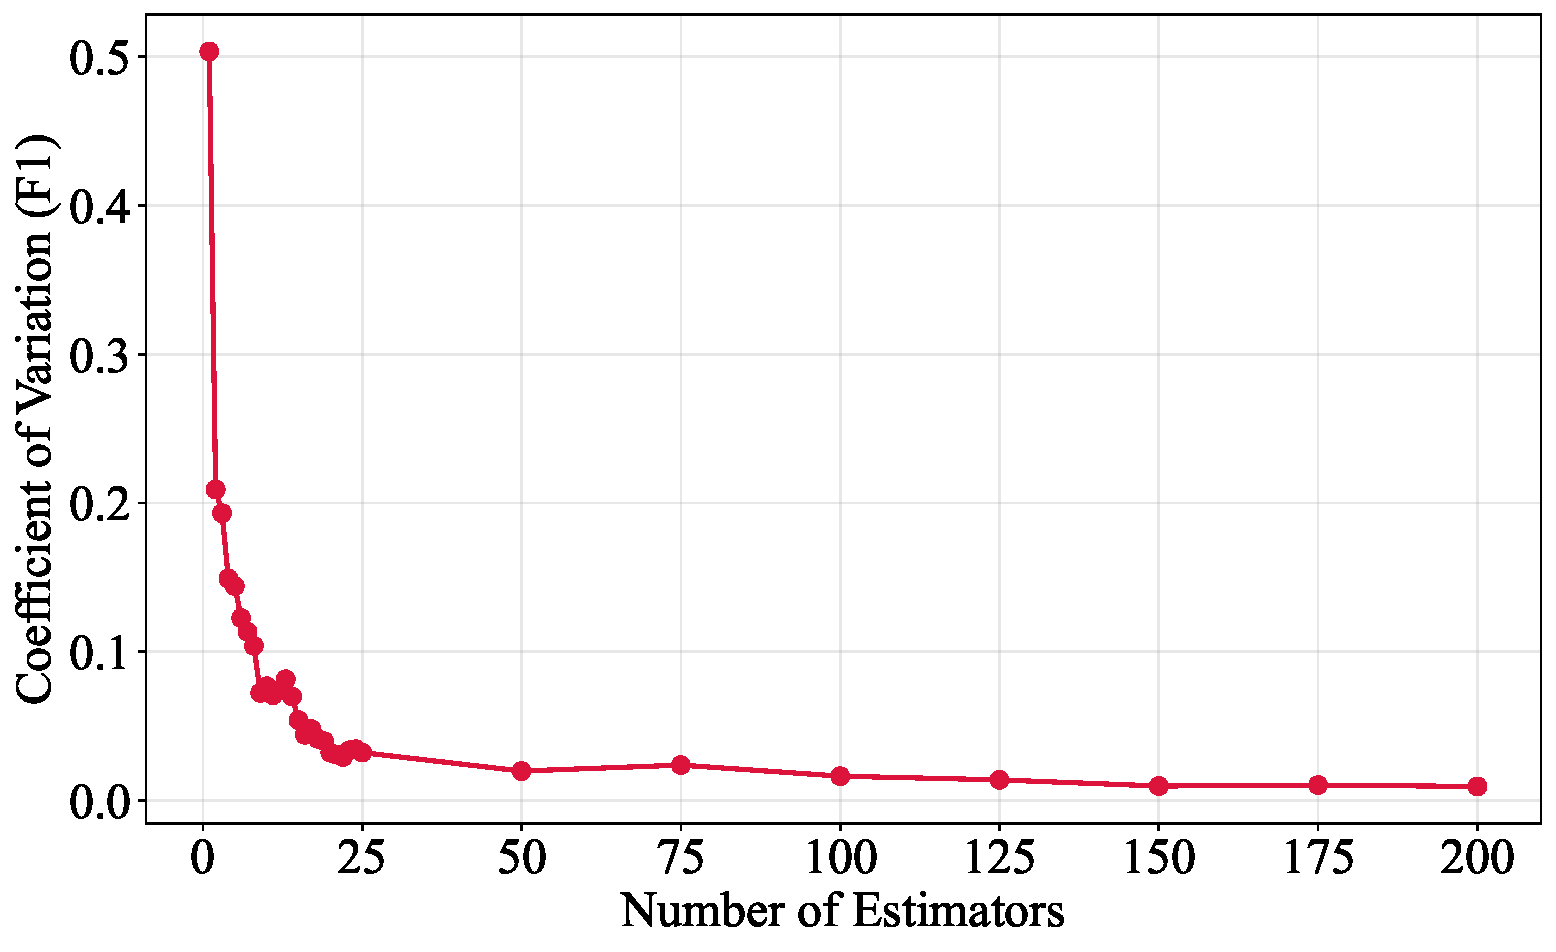
\includegraphics[width=\linewidth]{../results/shuttle/n_estimators/stability_analysis.pdf}
	\caption{Stability analysis of shuttle dataset.}
	\label{fig:n_estimators_var_shuttle}
\end{figure}
\begin{figure}[H]
	\centering
	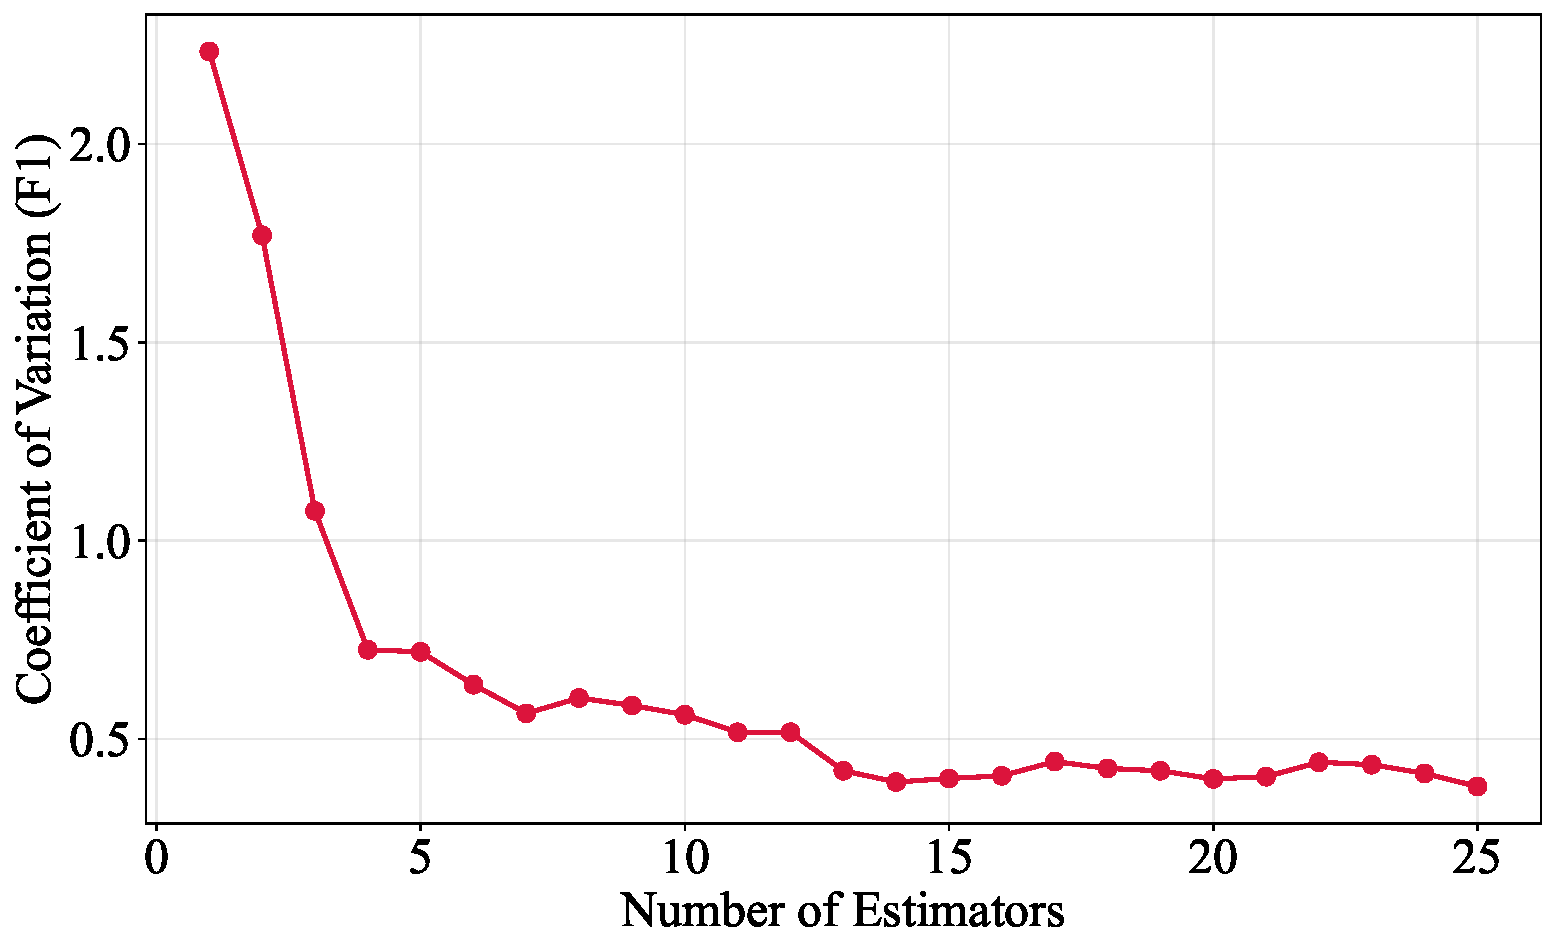
\includegraphics[width=\linewidth]{../results/fraud/n_estimators/stability_analysis.pdf}
	\caption{Stability analysis of fraud dataset.}
	\label{fig:n_estimators_var_fraud}
\end{figure}

\begin{figure}[H]
	\centering
	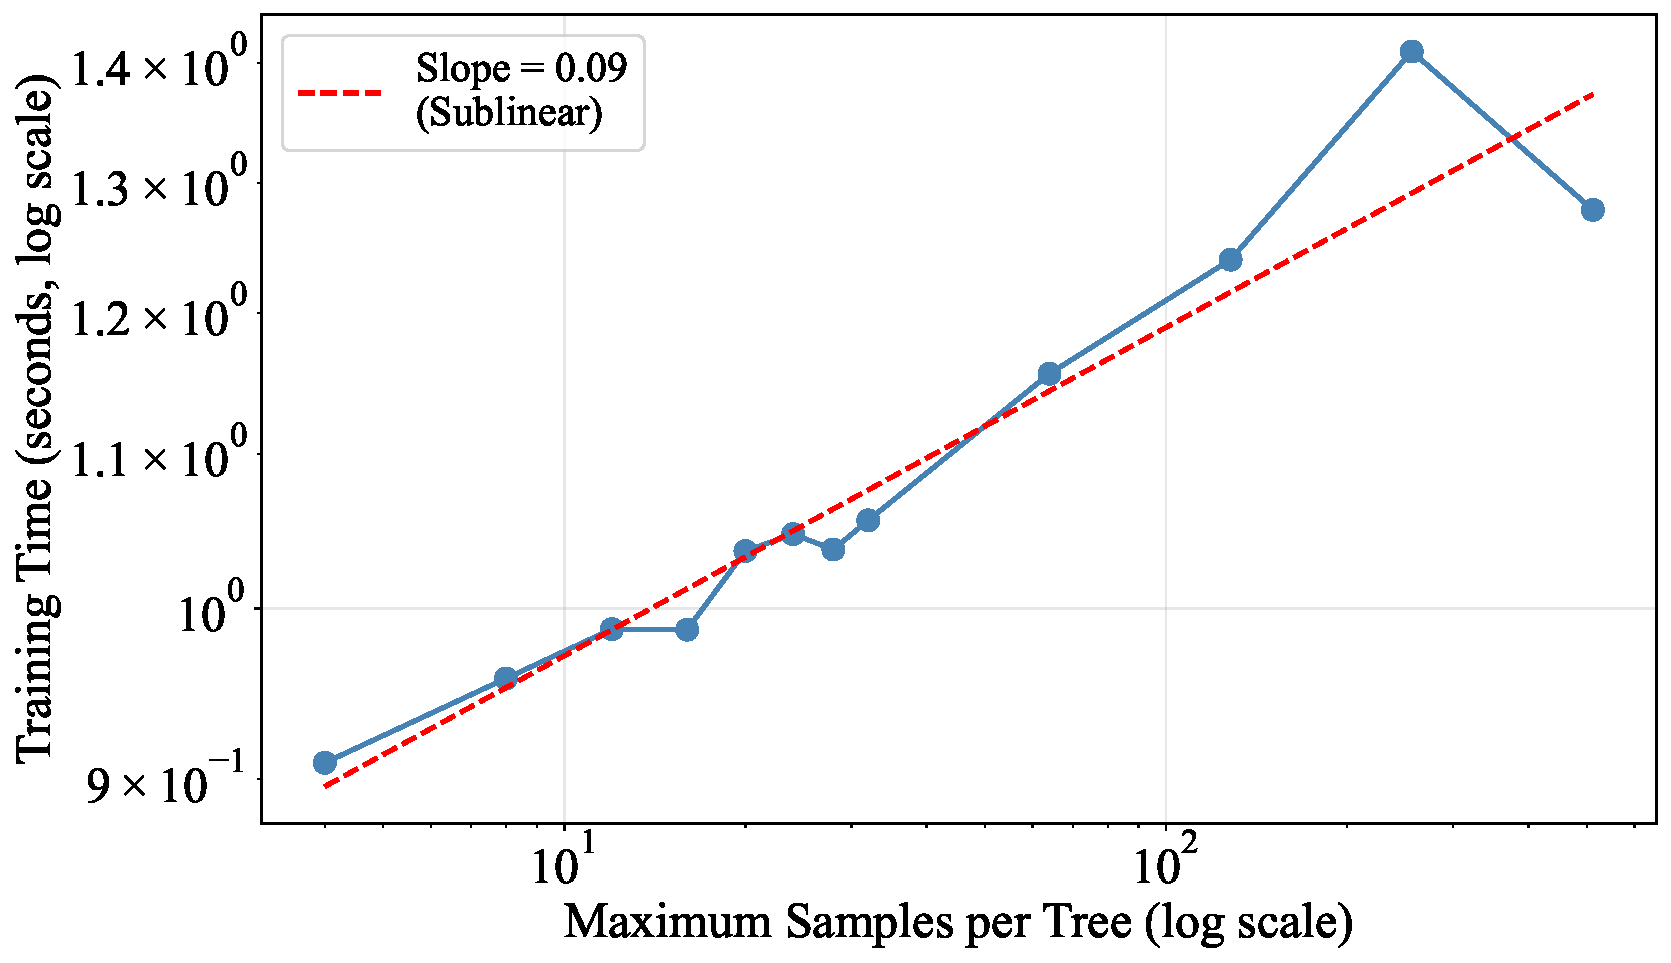
\includegraphics[width=0.95\linewidth]{../results/shuttle/max_samples/training_time_scaling.pdf}
	\caption{Training time scaling with maximum samples parameter for shuttle dataset.}
	\label{fig:tt_samples_shuttle}
\end{figure}
\begin{figure}[H]
	\centering
	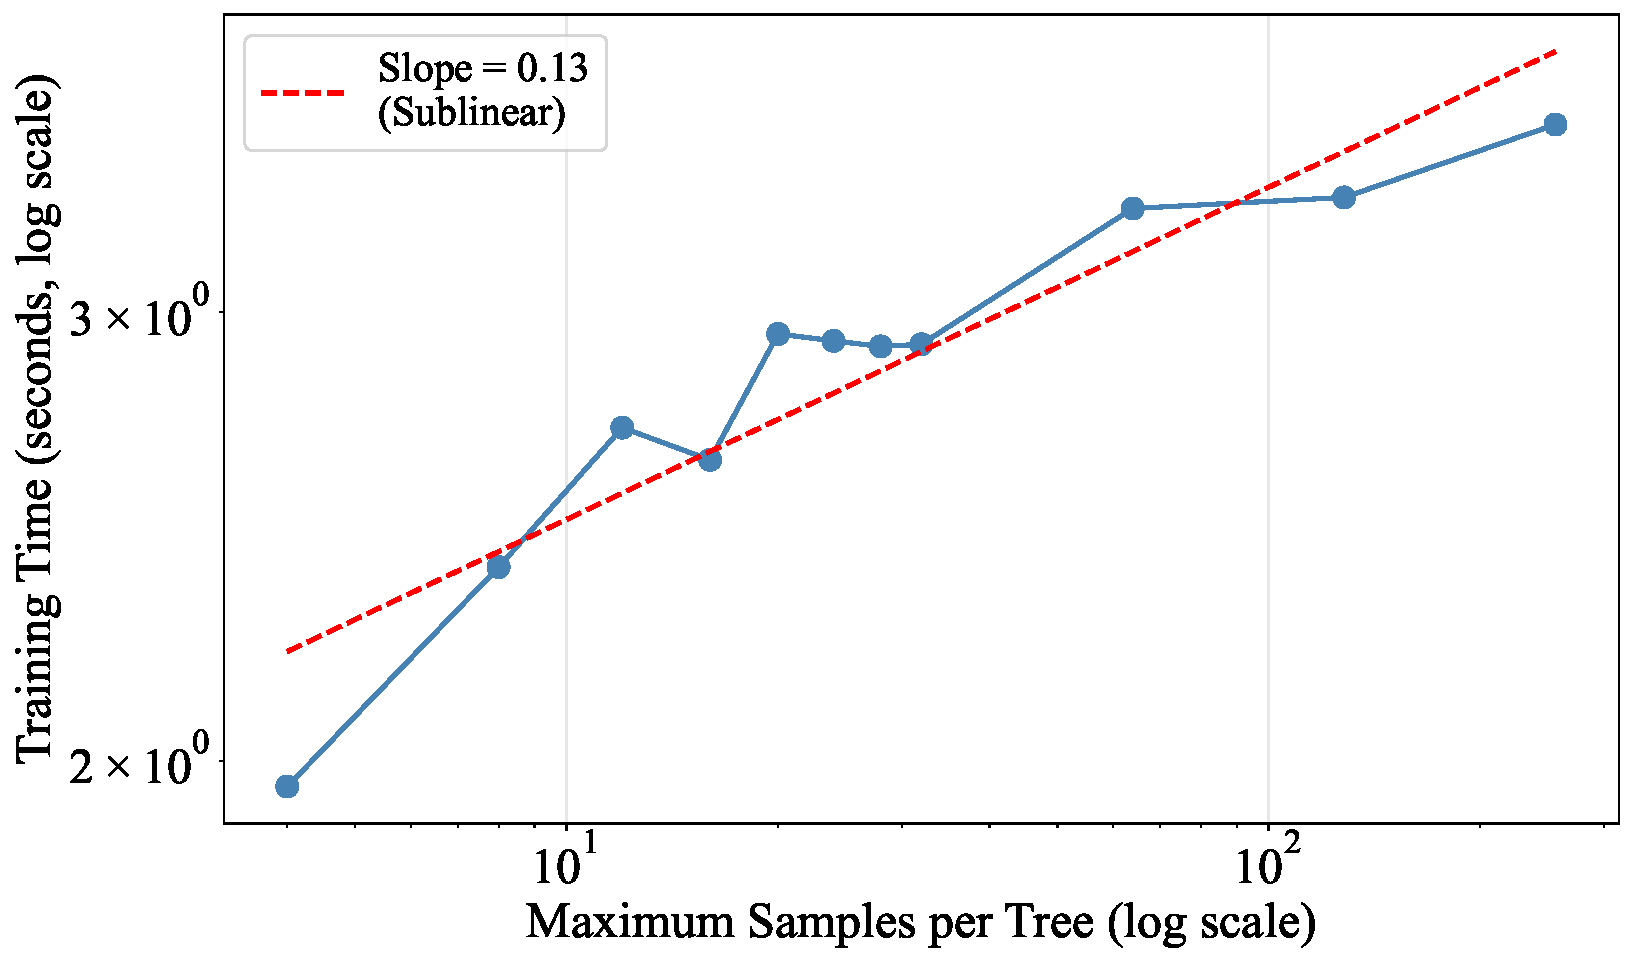
\includegraphics[width=0.95\linewidth]{../results/fraud/max_samples/training_time_scaling.pdf}
	\caption{Training time scaling with maximum samples parameter for fraud dataset.}
	\label{fig:tt_samples_fraud}
\end{figure}



\begin{figure}[H]
	\centering
	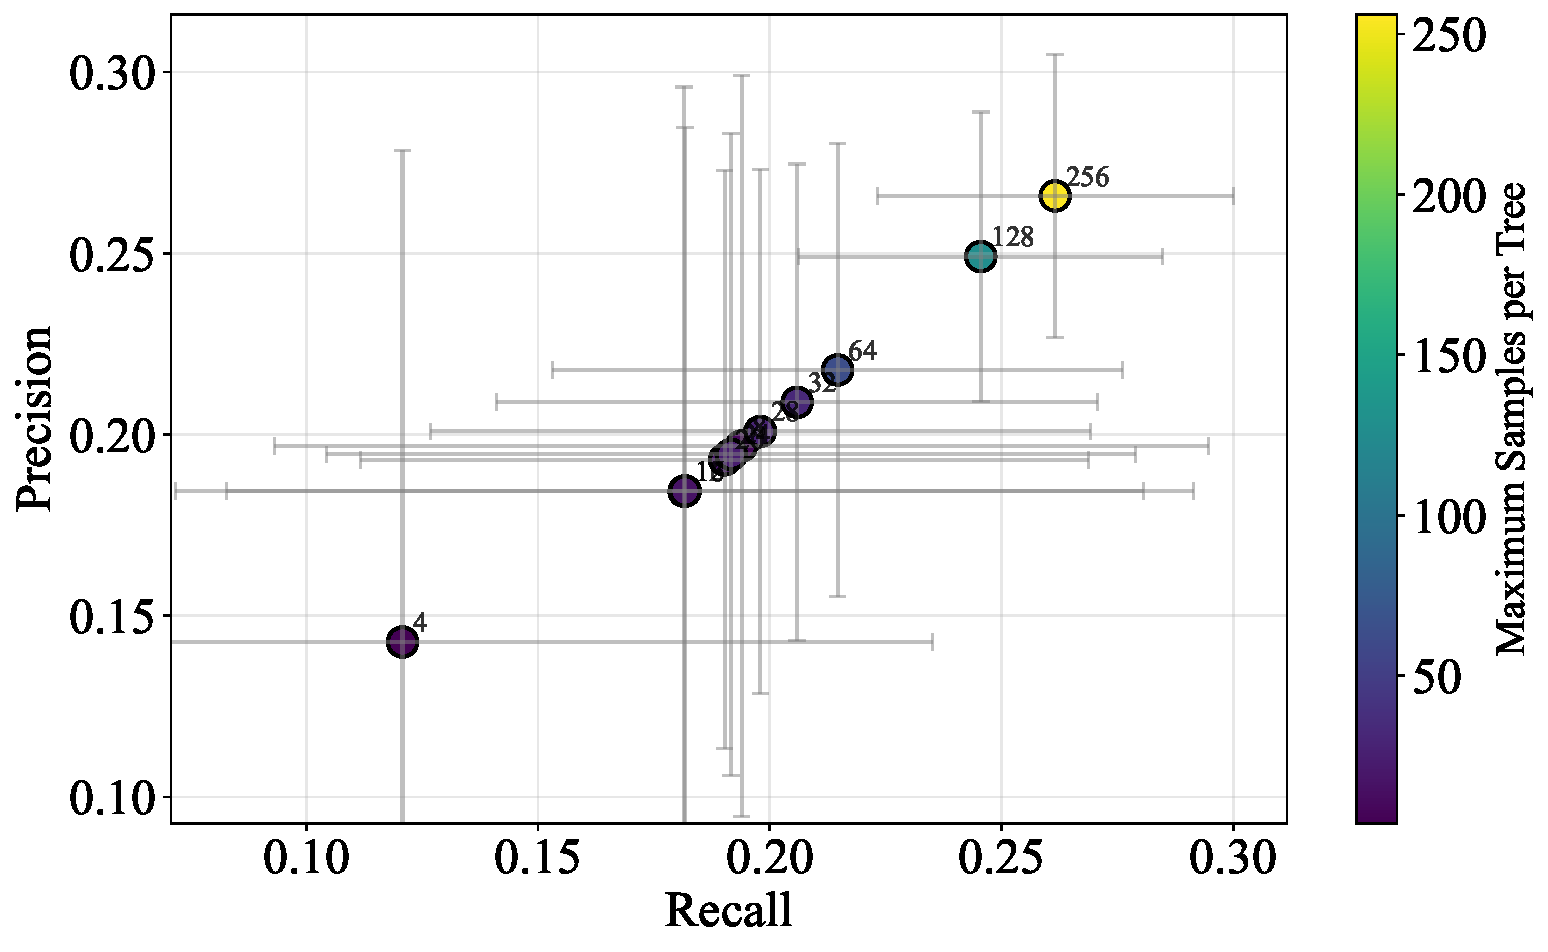
\includegraphics[width=\linewidth]{../results/fraud/max_samples/precision_recall_tradeoff.pdf}
	\caption{Precision recall trade-off for fraud dataset for various maximum sample parameters.}
	\label{fig:max_samples_fraud}
\end{figure}



\begin{figure}[H]
	\centering
	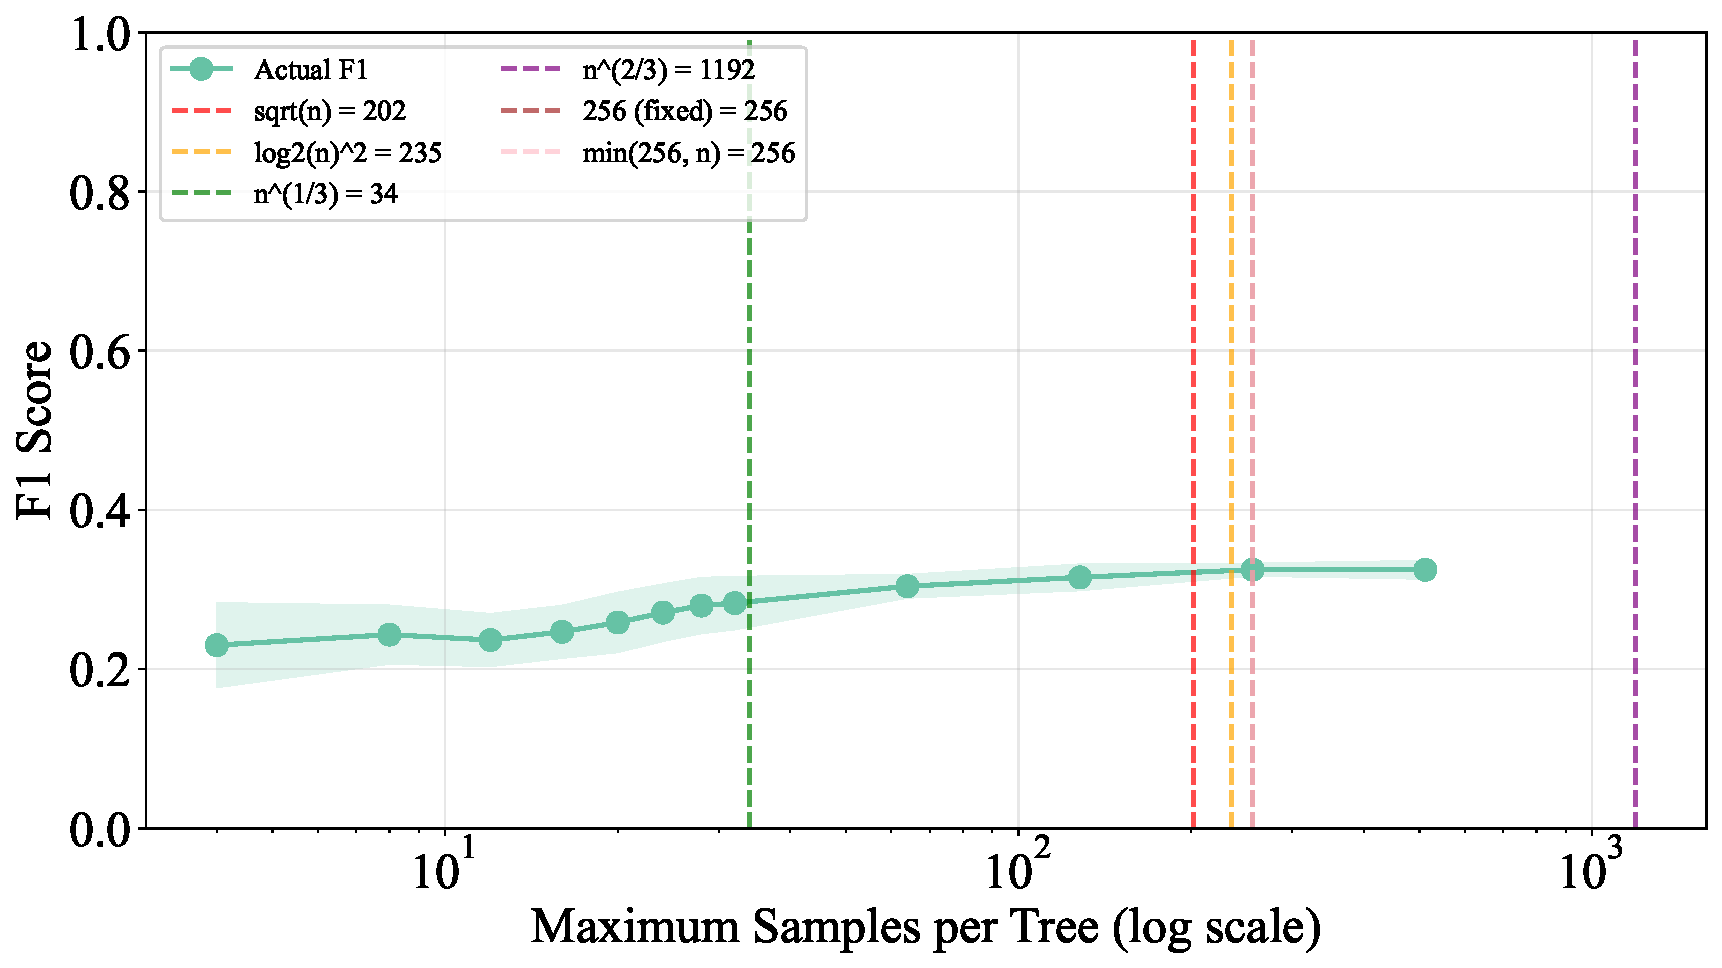
\includegraphics[width=0.95\linewidth]{../results/campaign/max_samples/empirical_rules.pdf}
	\caption{F1-score for various maximum samples parameter rules for campaign dataset.}
	\label{fig:rule_samples_campaign}
\end{figure}
\begin{figure}[H]
	\centering
	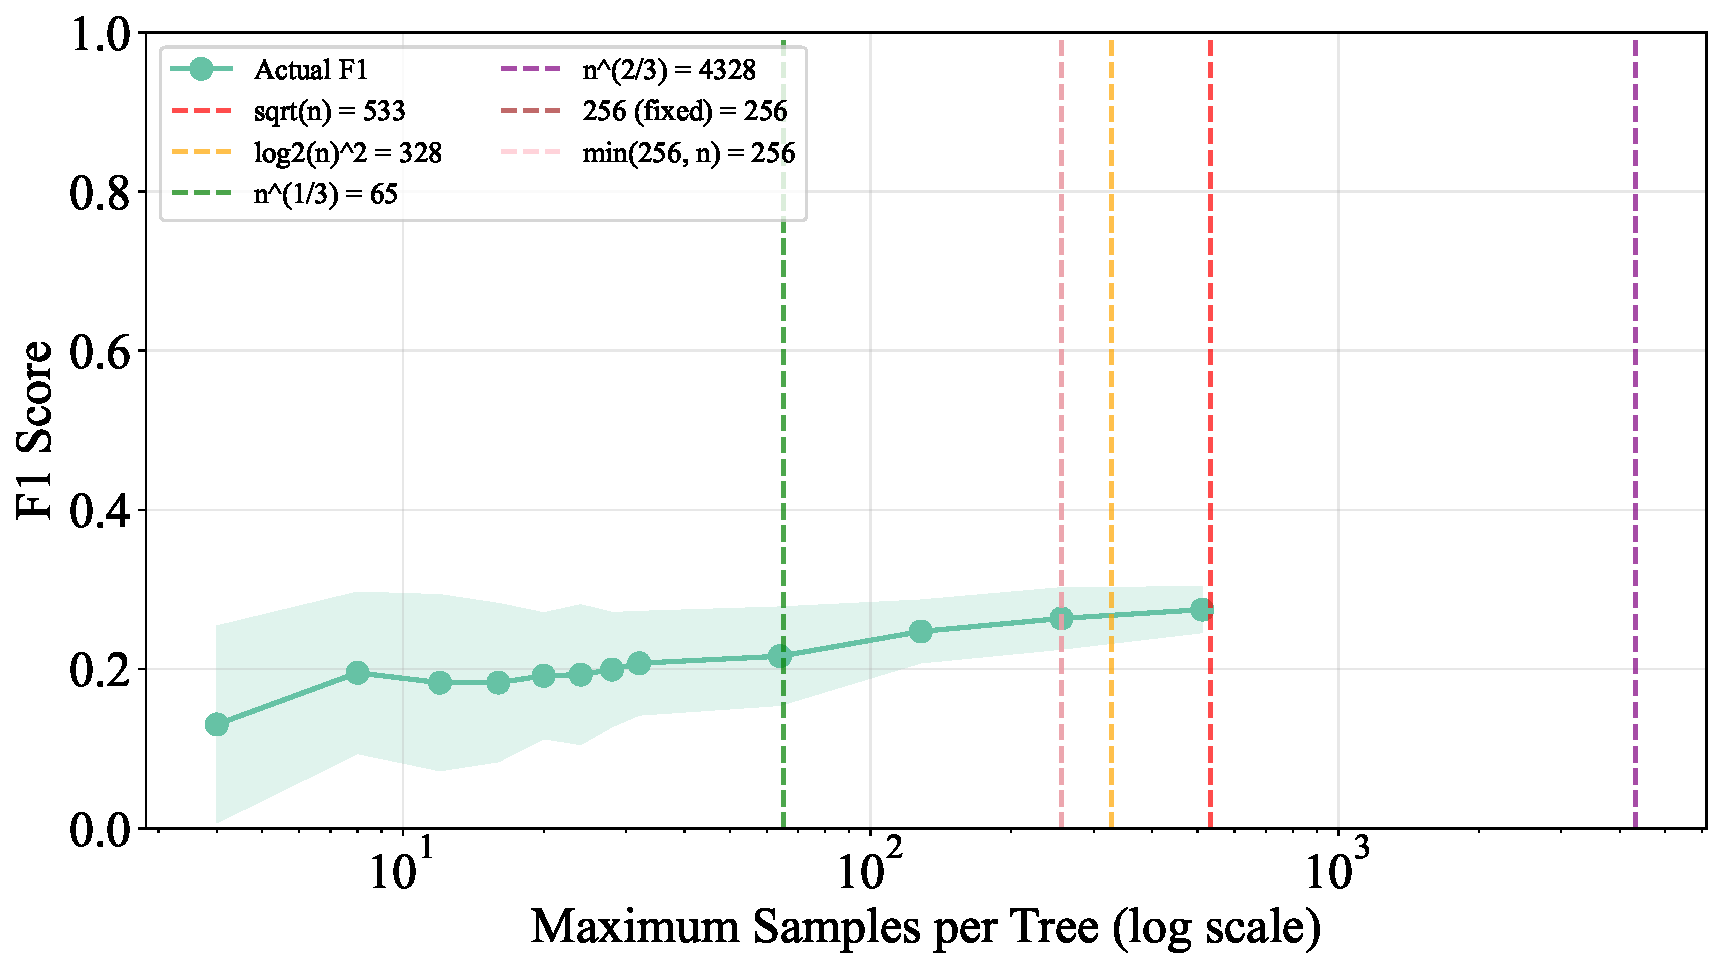
\includegraphics[width=0.95\linewidth]{../results/fraud/max_samples/empirical_rules.pdf}
	\caption{F1-score for various maximum samples parameter rules for fraud dataset.}
	\label{fig:rule_samples_fraud}
\end{figure}



\begin{figure}[H]
	\centering
	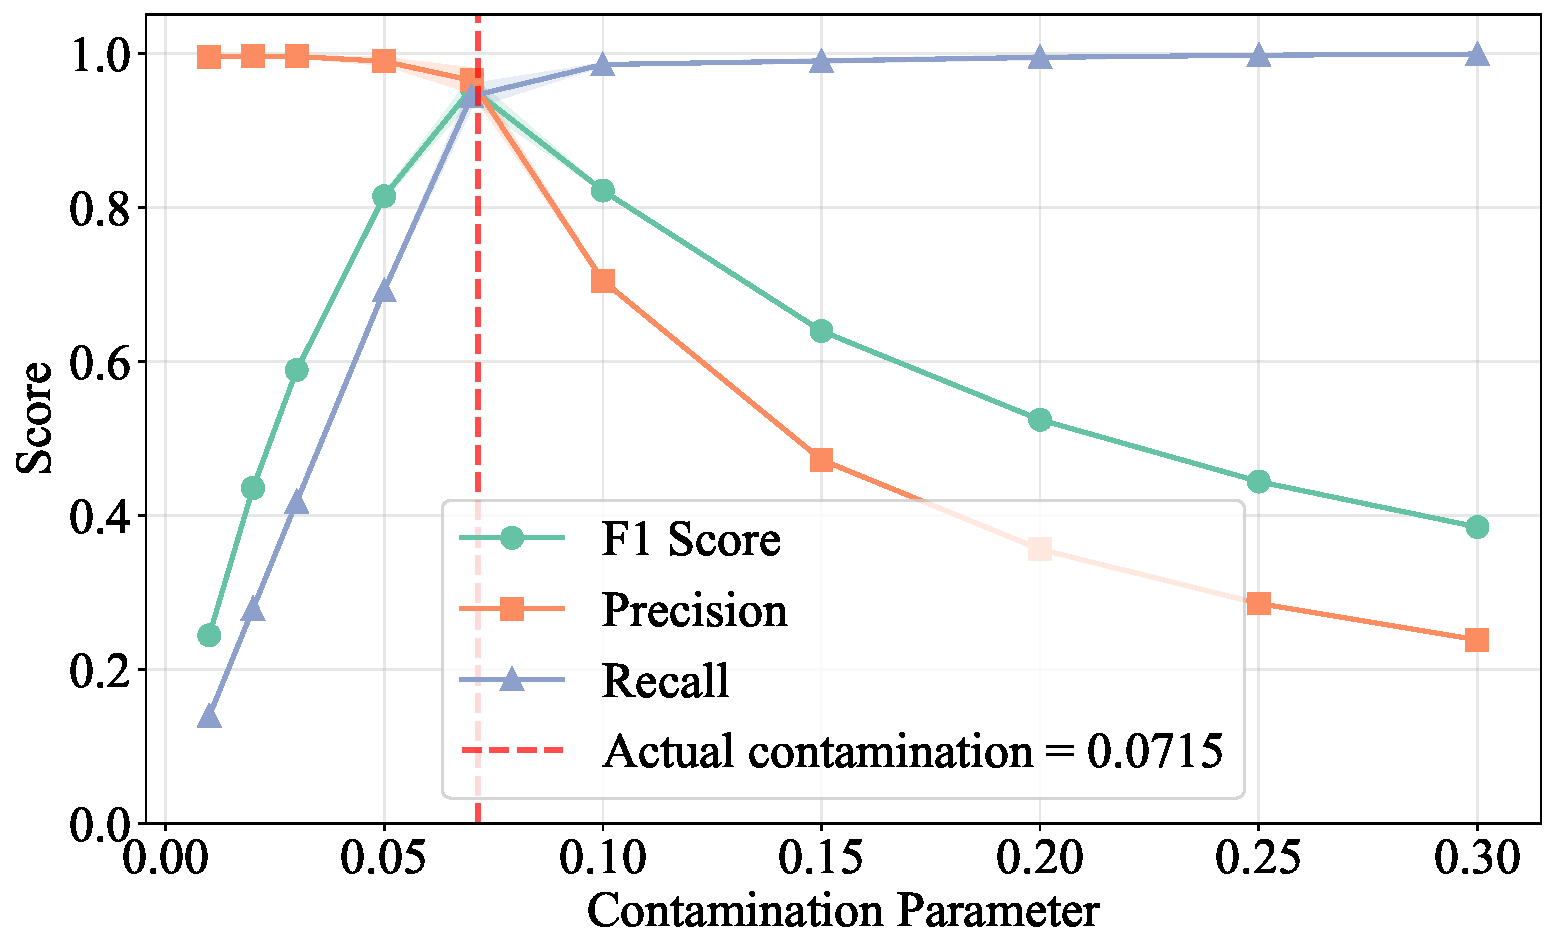
\includegraphics[width=0.95\linewidth]{../results/shuttle/contamination/performance_vs_contamination.pdf}
	\caption{Performance with increasing values of the contamination parameter for shuttle dataset.}
	\label{fig:contamination_shuttle}
\end{figure}



\begin{figure}[H]
	\centering
	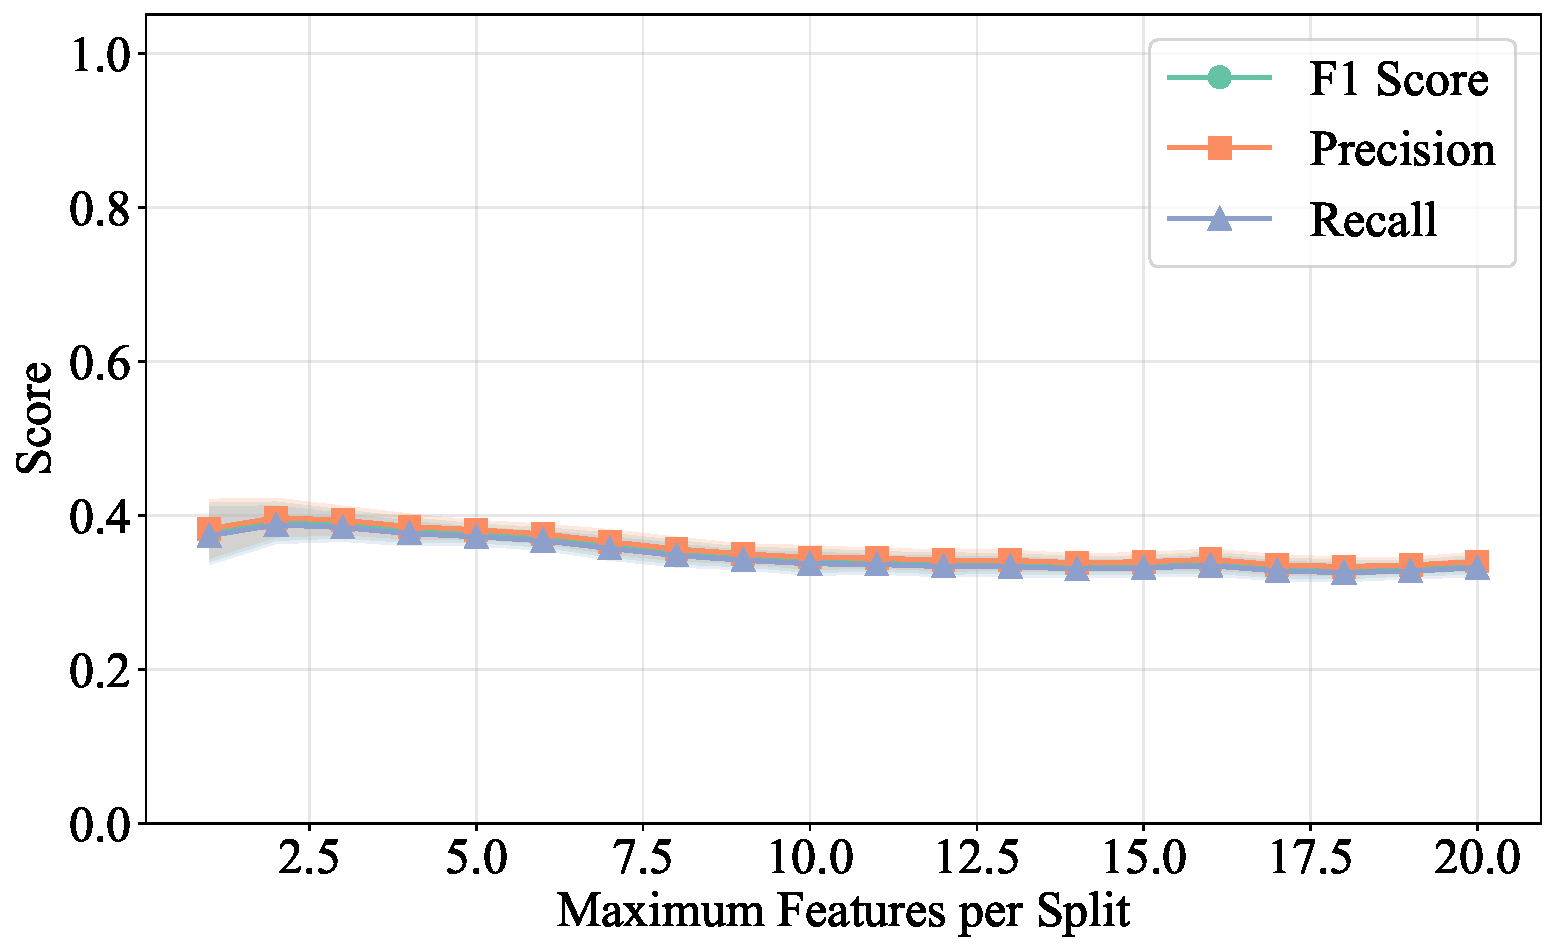
\includegraphics[width=0.95\linewidth]{../results/campaign/max_features/performance_vs_max_features.pdf}
	\caption{Performance of maximum features parameter for campaign dataset.}
	\label{fig:max_features_campaign}
\end{figure}

\begin{figure}[H]
	\centering
	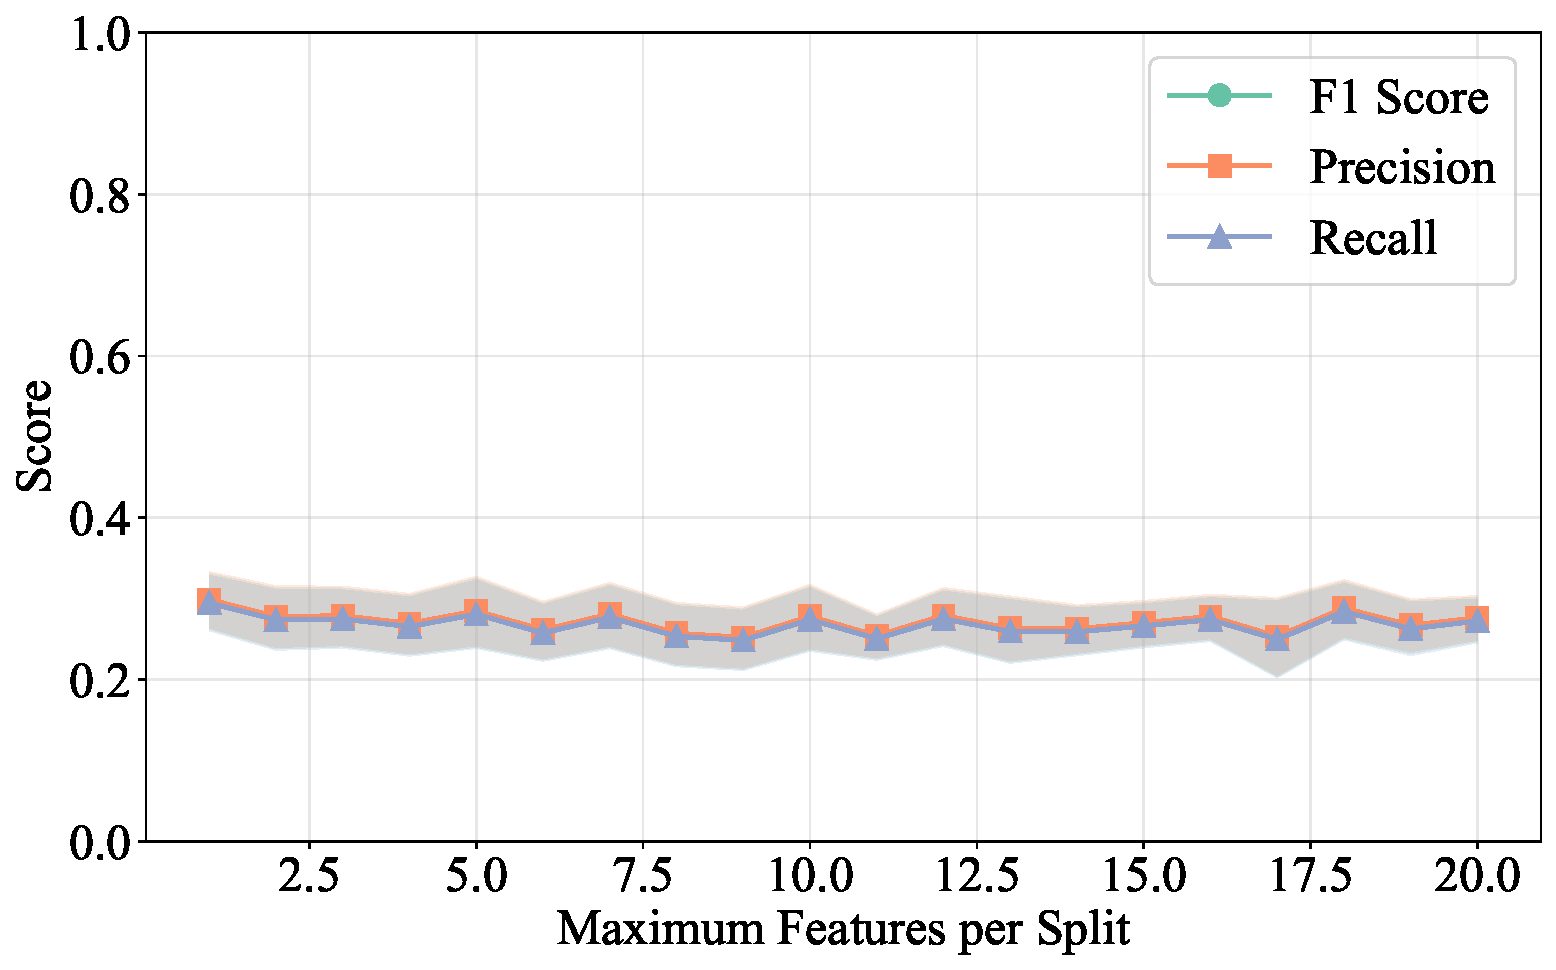
\includegraphics[width=0.95\linewidth]{../results/fraud/max_features/performance_vs_max_features.pdf}
	\caption{Performance of maximum features parameter for fraud dataset.}
	\label{fig:max_features_fraud}
\end{figure}



\begin{figure}[H]
	\centering
	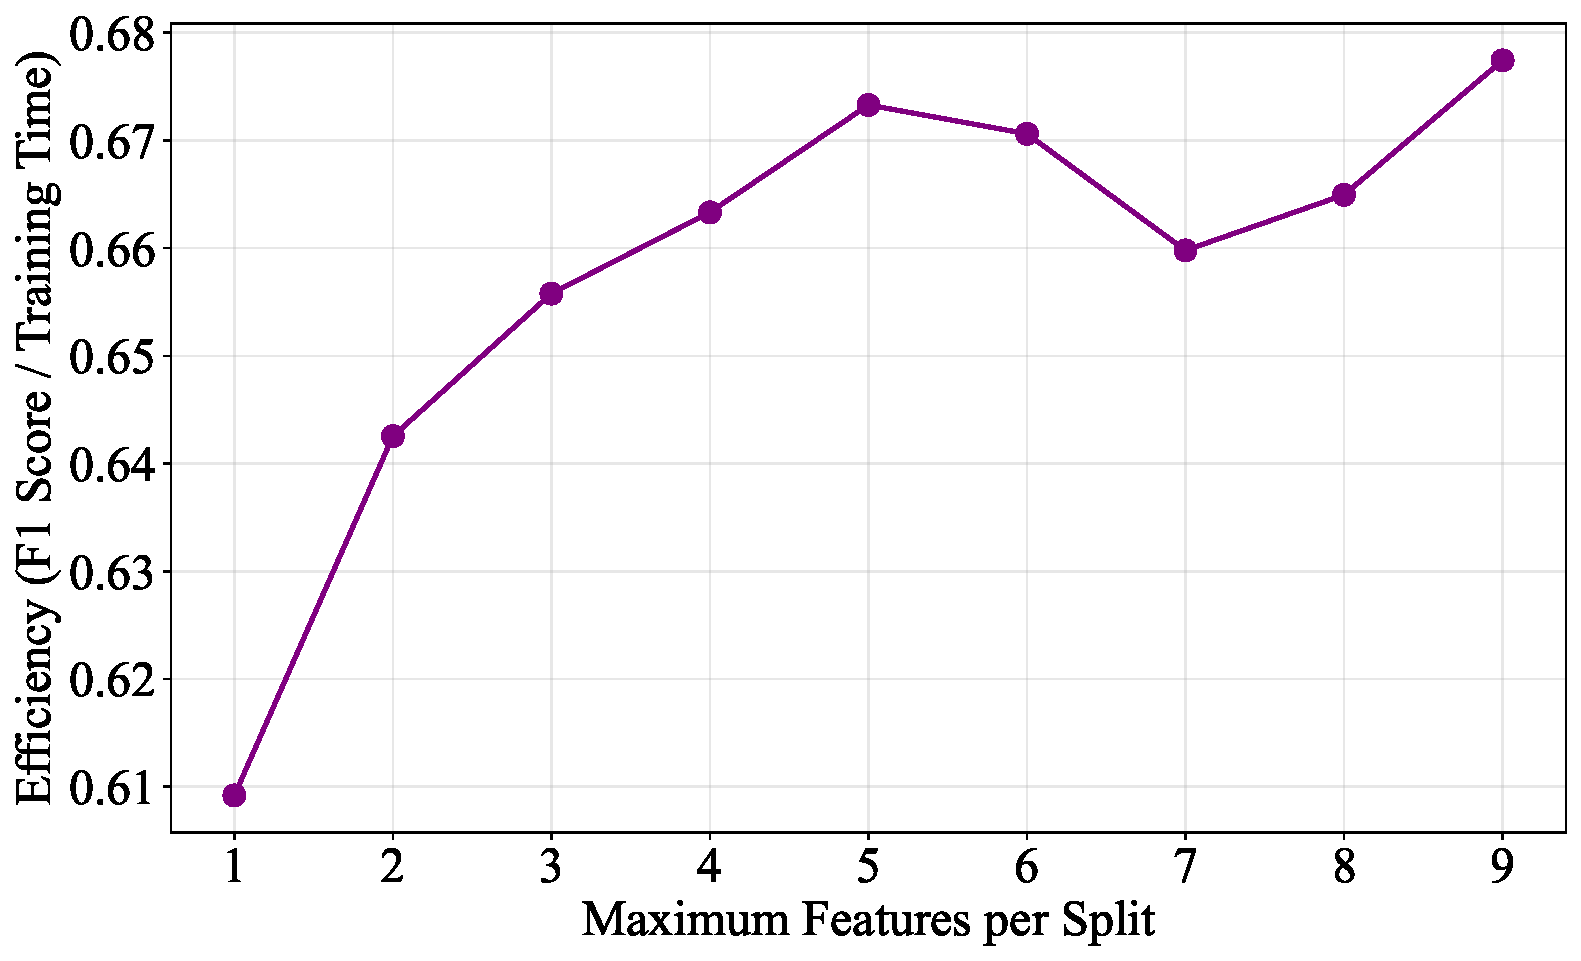
\includegraphics[width=0.95\linewidth]{../results/shuttle/max_features/efficiency_vs_max_features.pdf}
	\caption{Training time of maximum features parameter for shuttle dataset.}
	\label{fig:max_features_tt_shuttle}
\end{figure}
\begin{figure}[H]
	\centering
	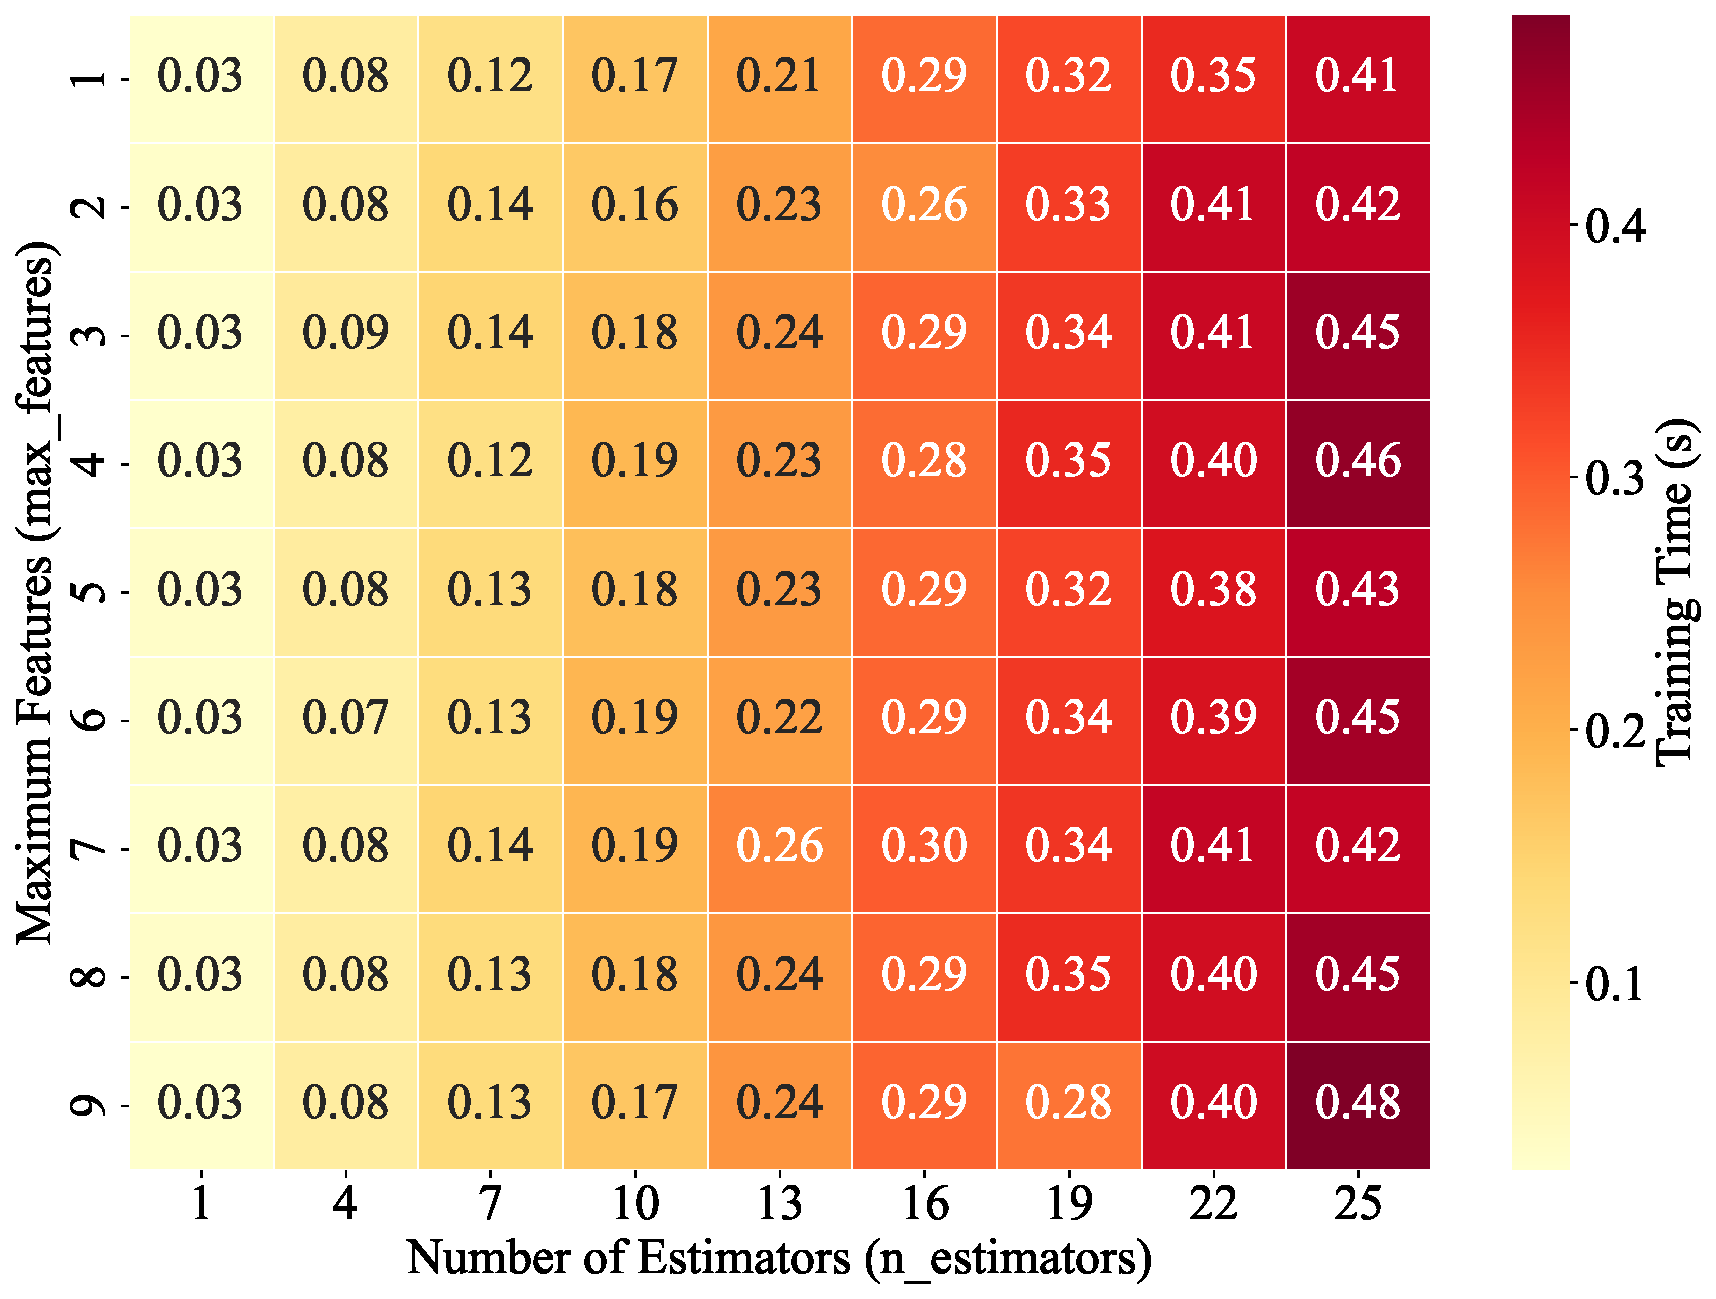
\includegraphics[width=0.95\linewidth]{../results/shuttle/max_features/interaction_time_heatmap.pdf}
	\caption{Interaction heatmap for number of features and estimators for shuttle dataset.}
	\label{fig:int_hm_tt_shuttle}
\end{figure}

\begin{figure}[H]
	\centering
	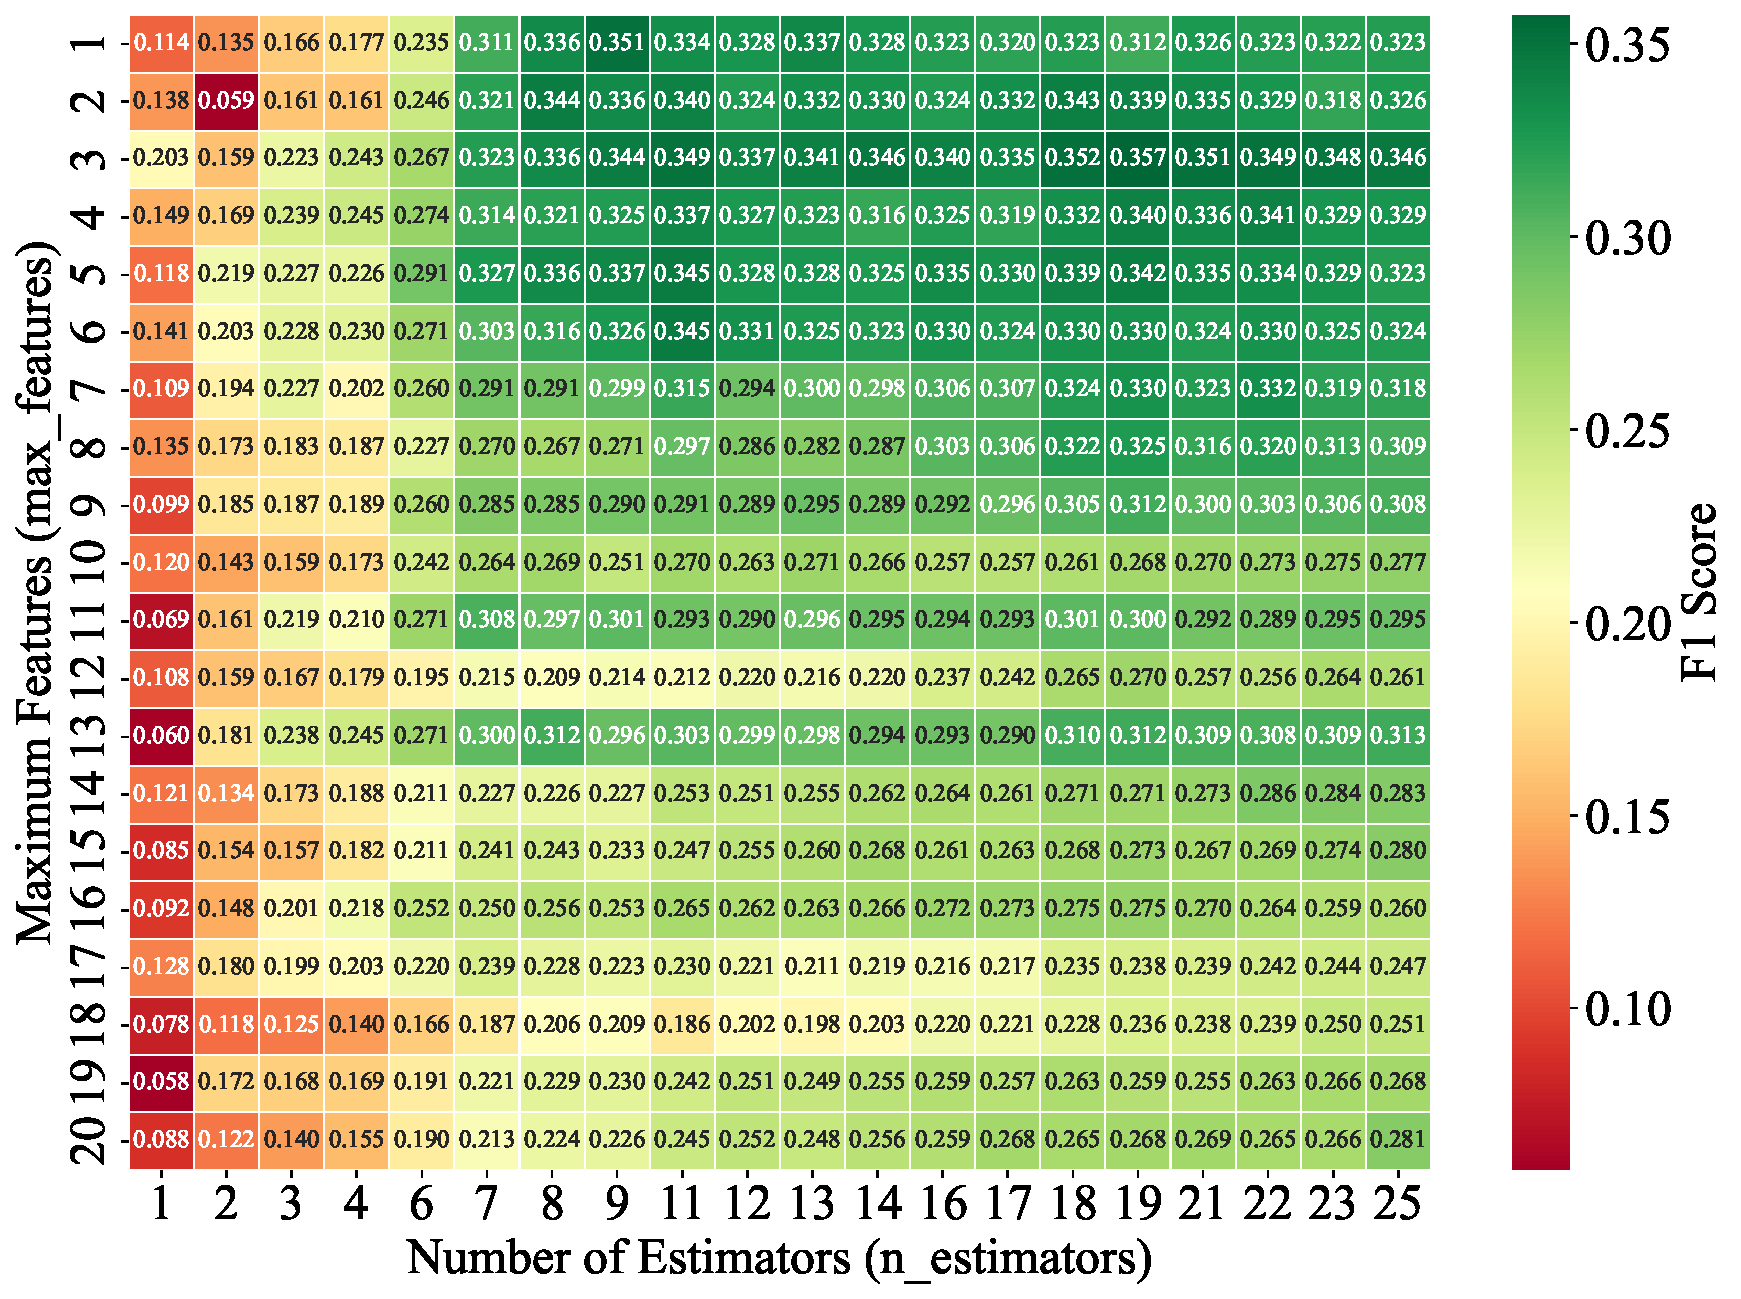
\includegraphics[width=0.95\linewidth]{../results/campaign/max_features/interaction_f1_heatmap.pdf}
	\caption{Interaction heatmap for number of features and estimators for campaign dataset.}
	\label{fig:int_hm_campaign}
\end{figure}



\begin{figure}[H]
	\centering
	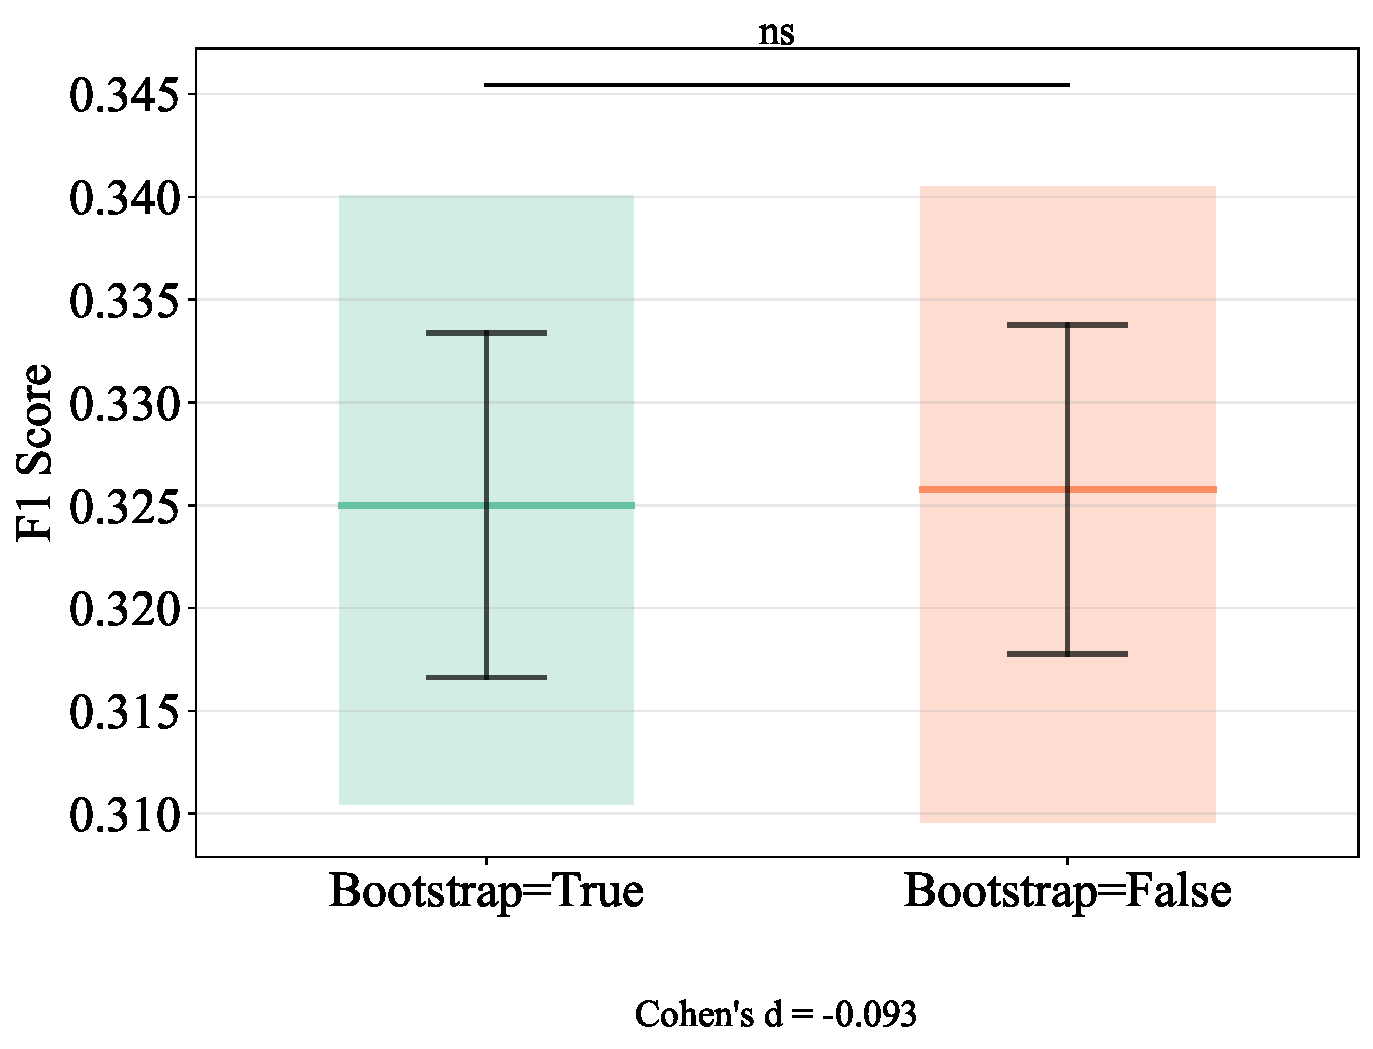
\includegraphics[width=0.95\linewidth]{../results/campaign/bootstrap/bootstrap_stability_box.pdf}
	\caption{Bootstrap stability for campaign dataset.}
	\label{fig:bootstrap_campaign}
\end{figure}

\begin{figure}[H]
	\centering
	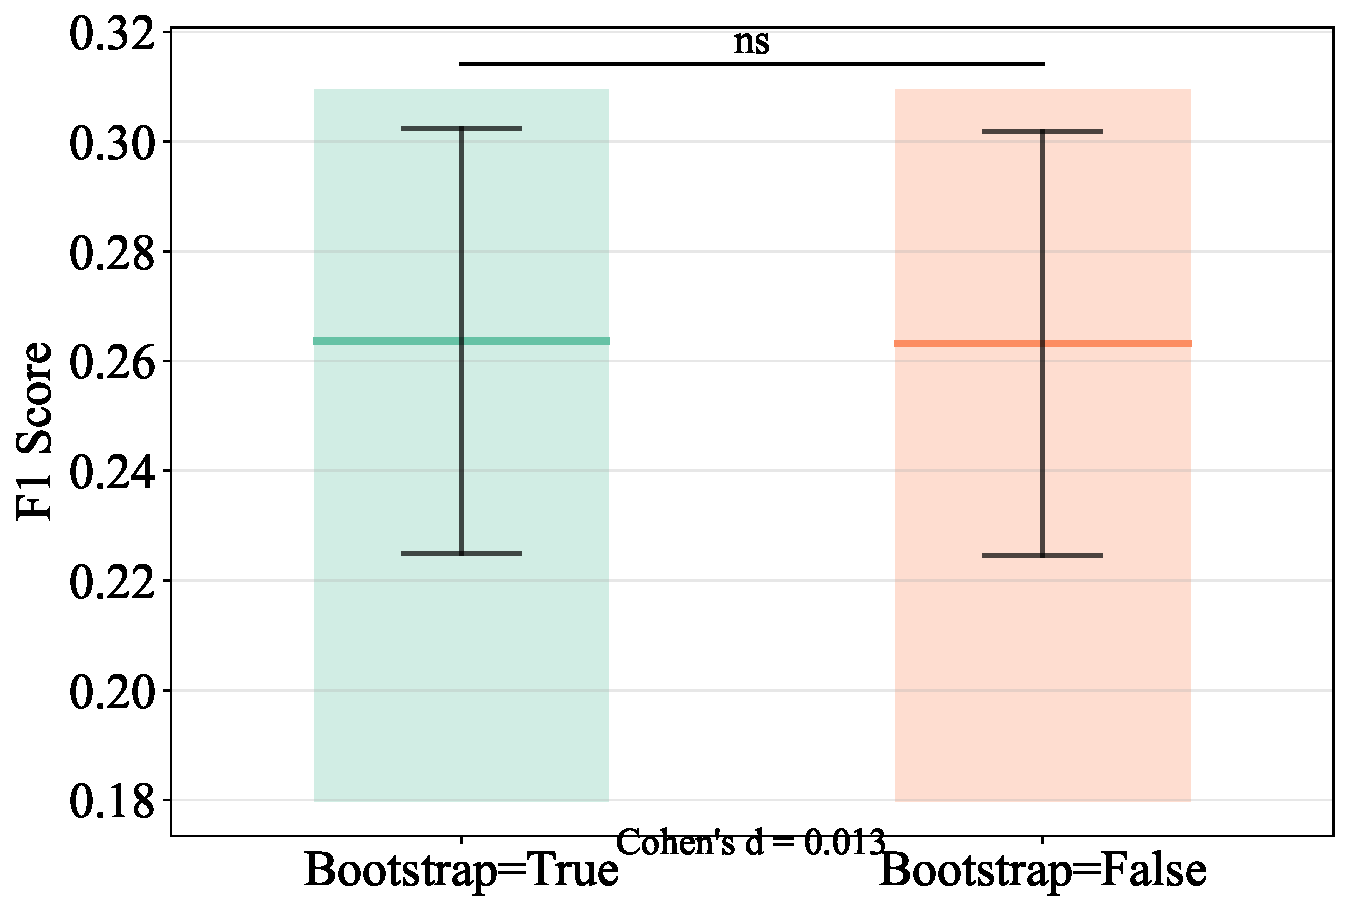
\includegraphics[width=0.95\linewidth]{../results/fraud/bootstrap/bootstrap_stability_box.pdf}
	\caption{Bootstrap stability for fraud dataset.}
	\label{fig:bootstrap_fraud}
\end{figure}


\end{document}
